\documentclass[journal,letterpaper]{IEEEtran}
\usepackage[letterpaper, left=0.65in, right=0.65in, bottom=0.7in, top=0.7in]{geometry}
\usepackage{stix}
\usepackage{siunitx}
\usepackage[version=4]{mhchem}
\usepackage{booktabs}
\usepackage{makecell}
\usepackage{multirow}
\usepackage{amsmath}
\usepackage{bm}
\usepackage{graphicx}
\usepackage{tikz}
\usepackage{pgfplots}
\usepackage{float}
\usepackage{fancyhdr}
\usepackage[none]{hyphenat}
\usepackage[hidelinks]{hyperref}
\usepackage{import}
\usepackage{transparent}
\usepackage{microtype}

\graphicspath{ {./figures/} }

\pgfplotsset{compat=1.18}

\setlength{\columnsep}{0.2in}
\setlength{\columnwidth}{3.5in}

\newlength\fheight
\newlength\fwidth
\setlength\fwidth{3.25in}
\setlength\fheight{0.8\fwidth}

\newcommand{\incfig}[1]{%
    \centering
    \def\svgwidth{3.5in}
    \import{./figures/}{#1.pdf_tex}
}

\renewcommand{\arraystretch}{1.3}

\sisetup{per-mode = symbol,
         inter-unit-product = \ensuremath{ { } \cdot { } },
         number-unit-product = \text{ },
         group-digits = false,
         detect-weight = true,
         detect-inline-weight = math,
         detect-display-math = true}

\pagestyle{fancy}
\fancyhf{}
\renewcommand{\headrulewidth}{0pt}
\rhead{\thepage}
\lhead{Section 11832 Lab 3}

\begin{document}
\title{Characterizing the Wake Region of a Smooth Cylinder}

\author{\IEEEauthorblockN{\LARGE{Borg, Auston J. \quad Lam, Brandon H. \quad Latzko, Alexander J. \\}}
\IEEEauthorblockA{
Section 11832 \quad October 10, 2023}
}

\maketitle
\thispagestyle{empty}

\begin{abstract}
This study presented a method of analyzing the effects of a cylinder in steady incompressible flow.
In addition to this, the Kármán vortex street was evaluated using four velocity power spectra to quantify the effect of the cylinder.
First, the hot wire anemometer was calibrated using ten data points while being placed in the middle of an empty test section at ten different fluid velocities.
Then, with the \qty{0.75}{in} diameter cylinder placed in the test section, the velocity of the flow was measured using the anemometer at seventeen different heights at the back of the test section.
The velocity at the centerline, top, and bottom of the cylinder were also measured.
The velocity data gathered at the center of the cylinder, top of the cylinder, edge of the wake, and outside the wake were then used to calculate a Strouhal number of $\bm{0.18 \pm 0.004}$ using the shedding frequency found through the generation of velocity power spectra.
It was found that the Strouhal number was only accurate when the velocity was not measured at the centerline of the cylinder due to the fluctuations in velocities being canceled at the center.
Using the previously generated velocity profile and numerical integration, the drag and drag coefficient on the cylinder was found to be $\bm{0.927 \pm }\mathbf{\qty{0.070}{\newton}}$ and $\bm{0.856 \pm 0.065}$, respectively, in a flow of Reynolds number $\bm{21000 \pm 938}$.
\end{abstract}

\begin{IEEEkeywords}
cylinder, hot wire anemometer, Kármán vortex street, wind tunnel
\end{IEEEkeywords}


\section{Introduction}


\IEEEPARstart{W}{hen} studying the aerodynamics of objects, an item of particular interest is the flow pattern around the object.
Analysis of the flow pattern can provide useful information about the object's flight characteristics such as the behavior of lift and drag.
When a bluff body is placed in steady uniform flow, the presence of the body disrupts the streamlines and typically causes flow separation behind the body, resulting in a turbulent wake.
The fluid velocity in the wake region can be characterized by a mean fluid velocity and perturbations that act in a cyclical manner.
These perturbations can be attributed to vortex shedding, called the Kármán vortex street, and have an associated frequency, $f$. To better quantify the frequency of this vortex shedding, a number called the Strouhal number relates the freestream velocity to the frequency and diameter of the object~\cite{Strouhal}.
This experiment had the objective of using a hot wire anemometer to determine the mean velocity profile and turbulent velocity profile in the wake of a smooth cylinder placed in the test section of a wind tunnel.
Additionally, the velocity spectra were found to at different points in the test section of the wind tunnel determine the vortex shedding frequency and corresponding Strouhal number.

The assumptions used to calculate the data in this report are that the fluid is incompressible, there is zero pressure gradient in the $x$-direction, and the flow is steady.
To record the fluid velocity at different points in the test section of the wind tunnel, a hot wire anemometer was used.
The hot wire anemometer functions by heating a thin wire placed in the test section.
As the air flows over the hot wire, convection heat transfer occurs and cools the wire.
Since the resistance of the wire is a function of the temperature of the wire, the cooling of the wire changes its resistance.
This results in a change in voltage that can be measured.
A hot wire anemometer was chosen for this experiment because it has a low time constant, meaning it is more sensitive to rapid velocity changes compared to other means of measuring air velocity.
This enables the capture of the Kármán vortex street.
The hot wire anemometer was calibrated with known freestream velocities to establish a fourth-order polynomial relationship between the measured voltage and the local fluid velocity.

With the calibrated hot wire anemometer, the local fluid velocity could be determined along different points in the wake of the cylinder.
First, the mean velocity profile in the wake of the cylinder was obtained.
Previous experiments with the wind tunnel have shown that the velocity profile of an unoccupied test section is approximately uniform except for at the walls of the wind tunnel~\cite{Lab1}.
Analysis of the mean velocity profile with the presence of the cylinder can demonstrate how bluff bodies disrupt the flow in the test section.
Disruptions in the flow would cause a drag force which can be measured with momentum conservation and the velocity data gathered for the velocity profile.
Equation~\eqref{eq:Drag} uses the momentum balance of the test section to calculate the total drag caused by the cylinder.
This integral was calculated through numerical integration where $q$ is the dynamic pressure, $U_2 (y)$ is the velocity at height $y$, $U_\infty$ is the freestream velocity, and $h$ is the height of the velocity profile~\cite{DragData}.
This drag force can then be non-dimensionalized using~\eqref{eq:Coeff} by dividing by its dynamic pressure $q$ and characteristic length $L$.

\begin{equation} \label{eq:Drag}
    F_D = q\int_{0}^{h} \frac{U_2 (y)}{U_\infty}2 \left(1 - \frac{U_2 (y)}{U_\infty}\right)\,dy
\end{equation}
\begin{equation} \label{eq:Coeff}
    C_D = \frac{F_D}{qL}
\end{equation}

Furthermore, previous research has shown that the amount of turbulence is directly correlated to the variance of the fluid velocity in the wake region behind the cylinder~\cite{Strouhal}.
With statistical samples of the fluid velocity, the standard deviation of the fluid velocities in the test section were plotted to obtain an understanding of the turbulent velocity profile.
Finally, spectrum analysis of the local fluid velocities at different locations should yield a dominant non-zero frequency in the flow.
This dominant frequency was determined to be the Strouhal frequency, from which the Strouhal number, $Sr$, of the flow could be calculated using~\eqref{eq:Strouhal}, where $f$ is the Strouhal frequency, $D$ is the body diameter, and $U_\infty$ is the freestream velocity~\cite{Strouhal}.
\begin{equation} \label{eq:Strouhal}
    Sr = \frac{fD}{U_\infty}
\end{equation}
The speed chosen to obtain the data necessary for the Strouhal number was chosen based on the predicted uncertainty in the calculation and the predicted behavior of the wake as seen in Fig.~\ref{fig:wake}.
The calculated Strouhal number was then compared with existing literature to best characterize the wake based on Fig.~\ref{fig:strouhal}. 

\begin{figure}[H]
    \centering
    \includegraphics[width=2.7in]{wake}
    \caption{Resulting wake behind a cylindrical body at various Reynolds numbers.}
    \label{fig:wake}
\end{figure}
\begin{figure}[H]
    \centering
    \includegraphics[width=3.4in]{Strouhal}
    \caption{Dimensionless shedding frequency (Strouhal number) as a function of Reynolds number~\cite{StrouhalPlot}.}
    \label{fig:strouhal}
\end{figure}

\section{Procedure}

\subsection{Calibrating the Hot Wire Anemometer}

Prior to the calibration of the hot wire anemometer, the ambient pressure, relative humidity, and ambient temperature were recorded.
The pressure transducer was calibrated to inches of water in the negative direction using the transducer's digital readout and a water manometer.
To calibrate the hot wire anemometer, the test section was emptied of all obstructions.
The hot wire anemometer was then moved to the middle of the test section height and lengthwise.
The calibration was taken over ten linearly spaced velocities.
The range of velocities measured was $7.54 \pm \qty{0.04}{\m\per\s}$ to $25.19 \pm \qty{0.04}{\m\per\s}$.
The wind tunnel was set to the corresponding static pressure for each velocity using the tunnel calibration coefficient determined from the first experiment.
At each calibration point, the voltage data from the anemometer and the pressure data from the pressure transducer were measured over 10 seconds at a sampling rate of \qty{2000}{\hertz}.

\subsection{Measuring the Velocity Profile}

A smooth brass cylinder of diameter 0.75 inches was placed into the test section.
The cylinder spanned across the test section width of 12 inches as seen in Fig.~\ref{fig:cylinder}.
The hot wire anemometer was moved to the back of the test section and was initially positioned to be \qty{8}{\cm} below the centerline of the cylinder.
At a Reynolds number of $21000 \pm 938$, the height of the anemometer was increased by \qty{1}{\cm} for each anemometer voltage measurement.
The height of the anemometer was increased to a maximum height of \qty{8}{\cm} above the centerline of the cylinder.
The voltage data for the seventeen data points were taken over 10 seconds at a sampling rate of \qty{2000}{\hertz}.
After collecting the seventeen data points, the anemometer voltage was taken at the top and bottom of the cylinder for the same sampling rate and time as the previous measurements.

\begin{figure}[H]
    \centering
    \includegraphics[width=2.9in]{Cylinder}
    \caption{Test section configuration for velocity profile measurement.}
    \label{fig:cylinder}
\end{figure}


\section{Results}

The ambient pressure, $P_\text{amb}$, of the room was measured using a wall-mounted barometer.
The temperature, $T$, and the relative humidity, $\varphi$, of the room was measured using a digital thermometer and hygrometer placed next to the test section.
The measured atmospheric conditions are summarized in Table~\ref{tab:atmCond}.

\begin{table}[H]
    \centering
    \caption{Atmospheric Conditions}
    \renewcommand{\arraystretch}{1.105}
    \begin{tabular}{ccc}
    \toprule
    Parameter & Value & Uncertainty ($\pm$) \\ \midrule \midrule
    $P_\text{amb}$ & \qty{762.60}{mm\ce{Hg}} & \qty{0.02}{mm\ce{Hg}} \\
    $T$ & \qty{21.9}{\celsius} & \qty{0.1}{\celsius} \\
    $\varphi$ & 51\% & 1\% \\ \bottomrule
    \end{tabular}
    \label{tab:atmCond}
\end{table}

The static gauge pressures measured using the pressure transducer were converted into the corresponding fluid velocities.
The pressures measures, where $P_\text{amb}$ is ambient pressure and $P_{ts}$ is test section pressure, are plotted against the voltages measured by the hot wire anemometer used during the calibration procedure in Fig.~\ref{fig:cal}.

\begin{figure}[H]
    \centering
    % This file was created by matlab2tikz.
%
%The latest updates can be retrieved from
%  http://www.mathworks.com/matlabcentral/fileexchange/22022-matlab2tikz-matlab2tikz
%where you can also make suggestions and rate matlab2tikz.
%
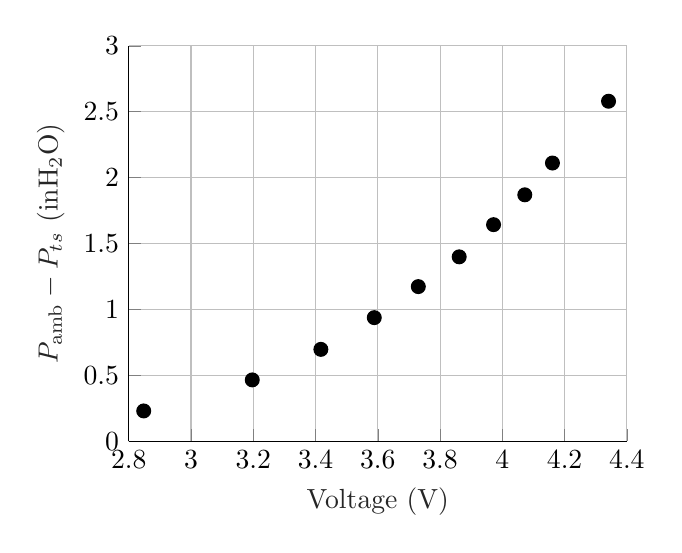
\begin{tikzpicture}

\begin{axis}[%
width=0.958\fwidth,
height=\fheight,
at={(0\fwidth,0\fheight)},
xmin=2.8,
xmax=4.4,
xlabel style={font=\color{white!15!black}},
xlabel={Voltage (V)},
ymin=0,
ymax=3,
ylabel style={font=\color{white!15!black}},
ylabel={$P_{\text{amb}} - P_{ts}$ (\unit{in\ce{H_2O}})},
ytick={0,0.5,...,3},
axis background/.style={fill=white},
axis x line*=bottom,
axis y line*=left,
xmajorgrids,
ymajorgrids
]
\addplot [color=black, only marks, mark size=2.5pt, mark=*, mark options={solid, black}, forget plot]
  table[row sep=crcr]{%
2.848186	0.230164\\
3.196808	0.46551\\
3.417166	0.697333\\
3.588717	0.937918\\
3.730116	1.173332\\
3.86145	1.399124\\
3.971786	1.643272\\
4.072112	1.869627\\
4.160987	2.110773\\
4.341081	2.579601\\
};
\end{axis}
\end{tikzpicture}%
    \caption{Hot wire anemometer calibration curve.}
    \label{fig:cal}
\end{figure}

The hot wire anemometer was then used to create a sample of 20000 data points at each of the sixteen positions behind the cylinder in the test section.
The mean of each voltage at each centimeter above and below was calculated and then tabulated with their respective uncertainties in Table~\ref{tab:voltage}.
A positive height is above the cylinder and a negative height is below the cylinder.
The mean voltage at the centerline, top and bottom of the cylinder were also taken with their values and uncertainties in Table~\ref{tab:voltages}.

\begin{table}[H]
    \centering
    \caption{Voltage Profile}
    \renewcommand{\arraystretch}{1.11}
    \begin{tabular}{cc}
    \toprule
    Height $h$ (cm) & Voltage $V$ (V) \\ \midrule \midrule
    $8.00 \pm 0.05 $ & $3.780 \pm 0.0002$ \\
    $7.00 \pm 0.05 $ & $3.777 \pm 0.0002$ \\
    $6.00 \pm 0.05 $ & $3.777 \pm 0.0004$ \\
    $5.00 \pm 0.05 $ & $3.768 \pm 0.0008$ \\
    $4.00 \pm 0.05 $ & $3.747 \pm 0.0012$ \\
    $3.00 \pm 0.05 $ & $3.721 \pm 0.0017$ \\
    $2.00 \pm 0.05 $ & $3.674 \pm 0.0020$ \\
    $1.00 \pm 0.05 $ & $3.577 \pm 0.0027$ \\
    $-1.00 \pm 0.05$ & $3.541 \pm 0.0028$ \\
    $-2.00 \pm 0.05$ & $3.646 \pm 0.0024$ \\
    $-3.00 \pm 0.05$ & $3.717 \pm 0.0018$ \\
    $-4.00 \pm 0.05$ & $3.742 \pm 0.0014$ \\
    $-5.00 \pm 0.05$ & $3.764 \pm 0.0010$ \\
    $-6.00 \pm 0.05$ & $3.780 \pm 0.0005$ \\
    $-7.00 \pm 0.05$ & $3.787 \pm 0.0003$ \\
    $-8.00 \pm 0.05$ & $3.785 \pm 0.0002$ \\ \bottomrule
    \end{tabular}
    \label{tab:voltage}
\end{table}

\begin{table}[H]
    \centering
    \caption{Voltage Profile (Cont.)}
    \begin{tabular}{ccc}
    \toprule
    Location & Height $h$ (cm) & Voltage $V$ (V) \\ \midrule \midrule
    Centerline & $0.00 \pm 0.05$ & $3.495 \pm 0.0030$ \\
    Top of Cylinder & $0.90 \pm 0.05$ & $3.532 \pm 0.0029$ \\
    Bottom of Cylinder & $-0.90 \pm 0.05$ & $3.583 \pm 0.0027$ \\ \bottomrule
    \end{tabular}
    \label{tab:voltages}
\end{table}


\section{Discussion}

\subsection{Hot Wire Anemometer Calibration}

From the ten calibration data points, a fourth-order polynomial was fit between the fluid velocity and the measured voltage (Fig.~\ref{fig:calCurve}).
This polynomial is shown by~\eqref{eq:poly}.
With the polynomial fit having a correlation coefficient of 0.9999, this indicated that the calibration curve fit well with the experimental data.
With the calibration curve, fluid velocities could be interpolated using the fourth-order polynomial and a measured voltage.

\begin{equation} \label{eq:poly}
    v = 0.0058V^4 - 0.894V^3 + 11.23V^2 - 34.95V + 35.97
\end{equation}

\begin{figure}[H]
    \centering
    % This file was created by matlab2tikz.
%
%The latest updates can be retrieved from
%  http://www.mathworks.com/matlabcentral/fileexchange/22022-matlab2tikz-matlab2tikz
%where you can also make suggestions and rate matlab2tikz.
%
\definecolor{mycolor1}{rgb}{0.65098,0.65098,0.65098}%
%
\begin{tikzpicture}

\begin{axis}[%
width=0.958\fwidth,
height=\fheight,
at={(0\fwidth,0\fheight)},
xmin=2.0,
xmax=4.5,
xlabel style={font=\color{white!15!black}},
xlabel={Voltage (V)},
ymin=0,
ymax=30,
ylabel style={font=\color{white!15!black}},
ylabel={Velocity (m/s)},
ytick={0,5,...,30},
axis background/.style={fill=white},
axis x line*=bottom,
axis y line*=left,
xmajorgrids,
ymajorgrids
]
\addplot [color=black, only marks, mark size=2.5pt, mark=*, mark options={solid, black}, forget plot]
  table[row sep=crcr]{%
2.848186	7.524611\\
3.196808	10.701145\\
3.417166	13.097422\\
3.588717	15.18966\\
3.730116	16.989322\\
3.86145	18.552126\\
3.971786	20.105755\\
4.072112	21.445843\\
4.160987	22.786963\\
4.341081	25.190799\\
};
\addplot [color=mycolor1, line width=2.5pt, forget plot]
  table[row sep=crcr]{%
2.848186	7.52217298535277\\
2.86326574747475	7.64205230170718\\
2.8783454949495	7.76367624901206\\
2.89342524242424	7.88702781646367\\
2.90850498989899	8.01209000051557\\
2.92358473737374	8.13884580487867\\
2.93866448484849	8.26727824052115\\
2.95374423232323	8.3973703256685\\
2.96882397979798	8.52910508580359\\
2.98390372727273	8.66246555366654\\
2.99898347474748	8.79743476925472\\
3.01406322222222	8.93399577982296\\
3.02914296969697	9.07213163988331\\
3.04422271717172	9.2118254112051\\
3.05930246464646	9.35306016281504\\
3.07438221212121	9.49581897099715\\
3.08946195959596	9.64008491929269\\
3.10454170707071	9.7858410985003\\
3.11962145454545	9.9330706066759\\
3.1347012020202	10.0817565491327\\
3.14978094949495	10.2318820384413\\
3.1648606969697	10.3834301944296\\
3.17994044444444	10.5363841441826\\
3.19502019191919	10.690727022043\\
3.21009993939394	10.8464419696104\\
3.22517968686869	11.003512135742\\
3.24025943434343	11.1619206765522\\
3.25533918181818	11.3216507554126\\
3.27041892929293	11.4826855429525\\
3.28549867676768	11.645008217058\\
3.30057842424242	11.8086019628729\\
3.31565817171717	11.9734499727982\\
3.33073791919192	12.1395354464919\\
3.34581766666667	12.3068415908699\\
3.36089741414141	12.475351620105\\
3.37597716161616	12.6450487556273\\
3.39105690909091	12.8159162261245\\
3.40613665656566	12.9879372675413\\
3.4212164040404	13.1610951230799\\
3.43629615151515	13.3353730431997\\
3.4513758989899	13.5107542856175\\
3.46645564646465	13.6872221153074\\
3.48153539393939	13.8647598045008\\
3.49661514141414	14.0433506326863\\
3.51169488888889	14.22297788661\\
3.52677463636364	14.4036248602751\\
3.54185438383838	14.5852748549424\\
3.55693413131313	14.7679111791297\\
3.57201387878788	14.9515171486123\\
3.58709362626263	15.1360760864227\\
3.60217337373737	15.3215713228509\\
3.61725312121212	15.507986195444\\
3.63233286868687	15.6953040490065\\
3.64741261616162	15.8835082356001\\
3.66249236363636	16.0725821145441\\
3.67757211111111	16.2625090524149\\
3.69265185858586	16.4532724230461\\
3.70773160606061	16.6448556075289\\
3.72281135353535	16.8372419942116\\
3.7378911010101	17.0304149786997\\
3.75297084848485	17.2243579638565\\
3.7680505959596	17.419054359802\\
3.78313034343434	17.614487583914\\
3.79821009090909	17.8106410608273\\
3.81328983838384	18.0074982224341\\
3.82836958585859	18.205042507884\\
3.84344933333333	18.4032573635839\\
3.85852908080808	18.6021262431979\\
3.87360882828283	18.8016326076474\\
3.88868857575758	19.0017599251112\\
3.90376832323232	19.2024916710254\\
3.91884807070707	19.4038113280835\\
3.93392781818182	19.6057023862361\\
3.94900756565657	19.8081483426912\\
3.96408731313131	20.0111327019141\\
3.97916706060606	20.2146389756276\\
3.99424680808081	20.4186506828115\\
4.00932655555556	20.6231513497032\\
4.0244063030303	20.8281245097971\\
4.03948605050505	21.0335537038453\\
4.0545657979798	21.2394224798568\\
4.06964554545455	21.4457143930981\\
4.08472529292929	21.6524130060932\\
4.09980504040404	21.8595018886231\\
4.11488478787879	22.0669646177262\\
4.12996453535354	22.2747847776984\\
4.14504428282828	22.4829459600925\\
4.16012403030303	22.6914317637192\\
4.17520377777778	22.9002257946459\\
4.19028352525253	23.1093116661978\\
4.20536327272727	23.3186729989571\\
4.22044302020202	23.5282934207633\\
4.23552276767677	23.7381565667135\\
4.25060251515151	23.9482460791619\\
4.26568226262626	24.15854560772\\
4.28076201010101	24.3690388092567\\
4.29584175757576	24.5797093478982\\
4.3109215050505	24.7905408950279\\
4.32600125252525	25.0015171292866\\
4.341081	25.2126217365723\\
};
\end{axis}
\end{tikzpicture}%
    \caption{Calibration graph for voltage velocity relation.}
    \label{fig:calCurve}
\end{figure}

The bounds of the fluid velocities used in the calibration were a minimum velocity of $7.54 \pm \qty{0.04}{\m\per\s}$ and a maximum velocity of $25.19 \pm \qty{0.04}{\m\per\s}$.
These bounds were selected so that during the determination of the velocity profile in the wake of the cylinder, the resulting fluid velocities were within the interpolation range of the calibration curve.
This allowed the construction of the velocity profile without extrapolation of data, minimizing systemic bias.
The uncertainty for the interpolated fluid velocities was obtained by using the greatest possible percent error from a combination of the uncertainty in the calibration fluid velocities and the random uncertainty in the hot wire anemometer itself.
See Appendix A for further details.

\subsection{Mean Fluid Velocity Profile}

The hot wire anemometer was placed throughout the height of the test section and the recorded voltages were interpolated to find the corresponding fluid velocities using the calibration curve.
The mean fluid velocity was then plotted against the position of the hot wire anemometer in the test section as seen in Fig.~\ref{fig:profile}.
There was a decrease in the mean fluid velocity in the wake of the cylinder with the flow reaching a minimum velocity directly behind the centerline of the cylinder.
This was likely due to the presence of the cylinder disrupting the streamlines behind the cylinder.
The mean fluid velocity when outside of the wake of the cylinder equalized around the intended freestream velocity of $17.67 \pm \qty{0.04}{\m\per\s}$.
Due to the relatively low uncertainty in the interpolated velocities, it can be judged that the shape of the mean velocity profile of the fluid flow in the test section of the wind tunnel generally matched with what was expected from turbulent flow theory~\cite{lab3doc}.

\begin{figure}[H]
    \centering
    % This file was created by matlab2tikz.
%
%The latest updates can be retrieved from
%  http://www.mathworks.com/matlabcentral/fileexchange/22022-matlab2tikz-matlab2tikz
%where you can also make suggestions and rate matlab2tikz.
%
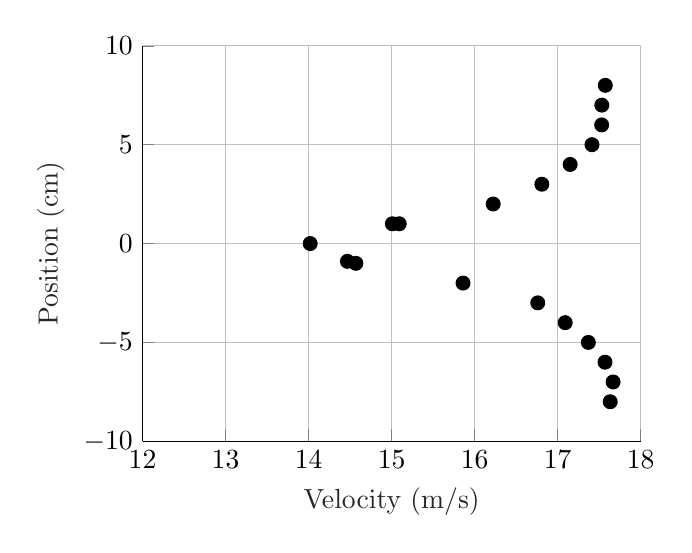
\begin{tikzpicture}

\begin{axis}[%
width=0.958\fwidth,
height=\fheight,
at={(0\fwidth,0\fheight)},
xmin=12,
xmax=18,
xlabel style={font=\color{white!15!black}},
xlabel={Velocity (m/s)},
ymin=-10,
ymax=10,
ylabel style={font=\color{white!15!black}},
ylabel={Position (cm)},
axis background/.style={fill=white},
axis x line*=bottom,
axis y line*=left,
xmajorgrids,
ymajorgrids
]
\addplot [color=black, only marks, mark size=2.5pt, mark=*, mark options={solid, black}, forget plot]
  table[row sep=crcr]{%
17.63302121	-8\\
17.66766483	-7\\
17.57029602	-6\\
17.36951483	-5\\
17.09044626	-4\\
16.76010295	-3\\
15.86014131	-2\\
14.5694144	-1\\
14.01914389	0\\
15.00864139	1\\
16.22321569	2\\
16.80958078	3\\
17.15024428	4\\
17.41338612	5\\
17.52997475	6\\
17.53175424	7\\
17.57363723	8\\
15.0918459	1\\
14.46785862	-0.9\\
};
\end{axis}
\end{tikzpicture}%
    \caption{Velocity profile behind a cylinder in uniform flow.}
    \label{fig:profile}
\end{figure}

\subsection{Turbulent Fluid Velocity Profile}

The standard deviation of the fluid velocities interpolated from the voltage of the hot wire anemometer was plotted against the position of the hot wire anemometer in the test section as seen in Fig.~\ref{fig:deviation}.
The standard deviation of the fluid velocity is directly correlated to the turbulence of the flow~\cite{turbulence}.
The turbulent fluid velocity profile indicates that the turbulence reached a maximum value when the hot wire anemometer was directly in line with the centerline of the cylinder.
The turbulence then diminished as the hot wire anemometer was moved further from the centerline of the cylinder and was minimum when outside of the wake flow of the cylinder.
The presence of a non-zero value for the standard deviation when outside of the wake flow could be attributed to the natural random uncertainty from recording voltages with the hot wire anemometer.
These findings matched previous literature that described how the flow behaves in the wake of a smooth cylinder~\cite{turbulence}.

\begin{figure}[H]
    \centering
    % This file was created by matlab2tikz.
%
%The latest updates can be retrieved from
%  http://www.mathworks.com/matlabcentral/fileexchange/22022-matlab2tikz-matlab2tikz
%where you can also make suggestions and rate matlab2tikz.
%
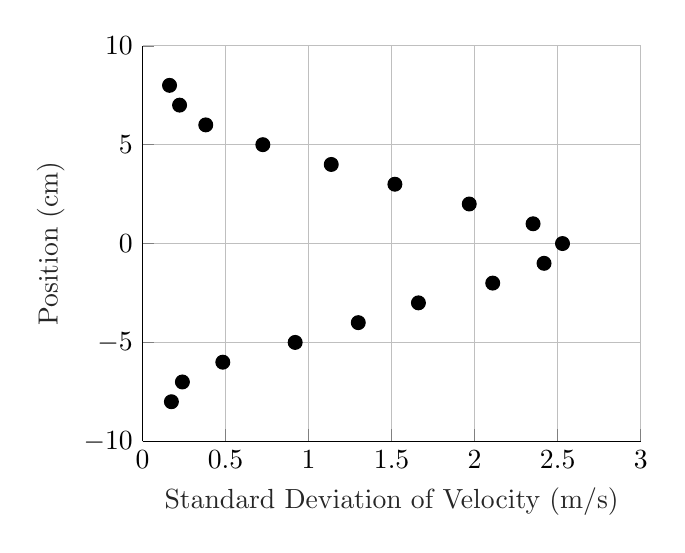
\begin{tikzpicture}

\begin{axis}[%
width=0.958\fwidth,
height=\fheight,
at={(0\fwidth,0\fheight)},
xmin=0,
xmax=3,
xlabel style={font=\color{white!15!black}},
xlabel={Standard Deviation of Velocity (m/s)},
ymin=-10,
ymax=10,
ylabel style={font=\color{white!15!black}},
ylabel={Position (cm)},
axis background/.style={fill=white},
axis x line*=bottom,
axis y line*=left,
xmajorgrids,
ymajorgrids
]
\addplot [color=black, only marks, mark size=2.5pt, mark=*, mark options={solid, black}, forget plot]
  table[row sep=crcr]{%
0.173818062	-8\\
0.239959547	-7\\
0.483283962	-6\\
0.919045562	-5\\
1.299192436	-4\\
1.661433296	-3\\
2.108859546	-2\\
2.417891131	-1\\
2.529128388	0\\
2.351792533	1\\
1.967515128	2\\
1.519674248	3\\
1.136372042	4\\
0.724403928	5\\
0.380683268	6\\
0.222989909	7\\
0.162576465	8\\
};
\end{axis}
\end{tikzpicture}%
    \caption{The standard deviation of the velocities measured in the test section.}
    \label{fig:deviation}
\end{figure}

\subsection{Drag Coefficient Calculation}

The drag of the cylinder was calculated through the conservation of momentum of a control volume and a numerical integration approximation.
Using~\eqref{eq:Drag} to numerically integrate over the entire profile, a drag force was found and is tabulated in Table~\ref{tab:Drag}.
This drag force could then be converted into a coefficient as seen in Table~\ref{tab:Drag} using~\eqref{eq:Coeff}.
The calculated coefficient of drag comes close to the theoretical drag coefficient for a cylinder of 1~\cite{dragRef}.
The error seen between the calculated coefficient and theoretical coefficient could be because of the resolution of the velocity profile.
By taking more data points, the numerical integration that was performed would be more accurate.
This would allow the coefficient to better match the expected theoretical drag coefficient more closely.

\begin{table}[H]
    \centering
    \caption{Drag on the Cylinder}
    \renewcommand{\arraystretch}{1.075}
    \begin{tabular}{ccc}
    \toprule
    Parameter & Value & Uncertainty ($\pm$) \\ \midrule \midrule
    $F_D$ & \qty{0.927}{\newton} & \qty{0.070}{\newton} \\
    $C_D$ & 0.856 & 0.065 \\ \bottomrule
    \end{tabular}
    \label{tab:Drag}
\end{table}

\subsection{Velocity Spectra}

To investigate the nature of the vortex shedding, a fast Fourier transform was used to take the discrete Fourier transform of the fluid velocities from the hot wire anemometer. Fig.~\ref{fig:freq2}, \ref{fig:freq3}, \ref{fig:freq4}, and \ref{fig:freq5} show the resulting velocity spectra of the data.

\begin{figure}[H]
    \centering
    % This file was created by matlab2tikz.
%
%The latest updates can be retrieved from
%  http://www.mathworks.com/matlabcentral/fileexchange/22022-matlab2tikz-matlab2tikz
%where you can also make suggestions and rate matlab2tikz.
%
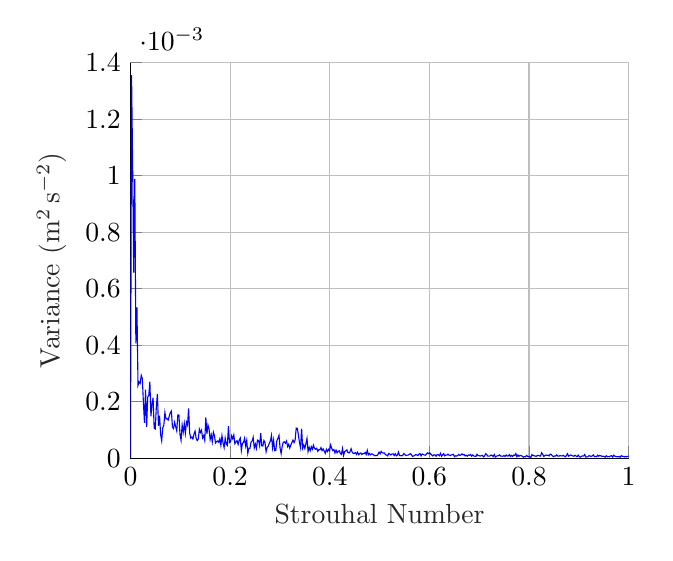
\begin{tikzpicture}

\begin{axis}[%
width=0.958\fwidth,
height=\fheight,
at={(0\fwidth,0\fheight)},
xmin=0,
xmax=1,
xlabel style={font=\color{white!15!black}},
xlabel={Strouhal Number},
ymin=0,
ymax=0.0014,
ylabel style={font=\color{white!15!black}},
ylabel={Variance (\unit{\m\squared\per\s\squared})},
ytick={0,0.0002,...,0.0014},
axis background/.style={fill=white},
axis x line*=bottom,
axis y line*=left,
xmajorgrids,
ymajorgrids
]
\addplot [color=blue, forget plot]
  table[row sep=crcr]{%
0	4.23400718544501e-31\\
0.0021605179799327	0.00135572708906543\\
0.0043210359598654	0.00103700171311617\\
0.0064815539397981	0.000656626543661401\\
0.0086420719197308	0.000988793771652281\\
0.0108025898996635	0.000406013755271573\\
0.0129631078795962	0.000533897579836336\\
0.0151236258595289	0.000257326604600796\\
0.0172841438394616	0.000269006605697543\\
0.0194446618193943	0.000264222950778624\\
0.021605179799327	0.000292789230368794\\
0.0237656977792597	0.000281674817711948\\
0.0259262157591924	0.000196945669628985\\
0.0280867337391251	0.000125088297616767\\
0.0302472517190578	0.000242321379894563\\
0.0324077696989905	0.000110651141566164\\
0.0345682876789232	0.000215967551486895\\
0.0367288056588559	0.000222051491853137\\
0.0388893236387886	0.000270540643360944\\
0.0410498416187213	0.000148144681819685\\
0.043210359598654	0.000190123586381455\\
0.0453708775785867	0.000213913797647736\\
0.0475313955585194	0.000106645633356474\\
0.0496919135384521	0.000103186158593583\\
0.0518524315183848	0.000179215709177537\\
0.0540129494983175	0.000227230378635952\\
0.0561734674782502	0.0001144572336935\\
0.0583339854581829	0.000150325393273142\\
0.0604945034381156	8.3246690729388e-05\\
0.0626550214180483	6.12747086485669e-05\\
0.064815539397981	0.000107531918901703\\
0.0669760573779137	0.000116827509960682\\
0.0691365753578464	0.000161300261646291\\
0.0712970933377791	0.000138619375245062\\
0.0734576113177118	0.00014009381221374\\
0.0756181292976445	0.000134533248514906\\
0.0777786472775772	0.000148277790723557\\
0.0799391652575099	0.000160759602895038\\
0.0820996832374426	0.000166390986027641\\
0.0842602012173753	0.000110118897998614\\
0.086420719197308	0.000104489732405442\\
0.0885812371772407	0.000126564704112698\\
0.0907417551571734	0.00011144280097919\\
0.0929022731371061	9.60826679589994e-05\\
0.0950627911170388	0.000153095798604959\\
0.0972233090969715	0.000153106522156094\\
0.0993838270769042	8.33444982323682e-05\\
0.101544345056837	6.29560441048174e-05\\
0.10370486303677	0.000116810699183991\\
0.105865381016702	9.18388579707487e-05\\
0.108025898996635	0.000122545093785624\\
0.110186416976568	8.82443097270251e-05\\
0.1123469349565	0.000127588801894074\\
0.114507452936433	0.000116973287319633\\
0.116667970916366	0.000175671821461894\\
0.118828488896299	8.91907077317363e-05\\
0.120989006876231	7.07351487087738e-05\\
0.123149524856164	7.45653928782151e-05\\
0.125310042836097	6.77665812437785e-05\\
0.127470560816029	8.53016523237154e-05\\
0.129631078795962	9.54813076866011e-05\\
0.131791596775895	6.98291166809875e-05\\
0.133952114755827	6.20349352004595e-05\\
0.13611263273576	6.76614688947983e-05\\
0.138273150715693	0.000102274852823817\\
0.140433668695626	9.05341606579586e-05\\
0.142594186675558	9.88164001895583e-05\\
0.144754704655491	7.12806007479651e-05\\
0.146915222635424	7.93800723001957e-05\\
0.149075740615356	6.29767378798622e-05\\
0.151236258595289	0.000143952151551626\\
0.153396776575222	8.55848524418719e-05\\
0.155557294555154	0.000116818017455421\\
0.157717812535087	0.000102778739498806\\
0.15987833051502	6.56537588104546e-05\\
0.162038848494953	8.25798821406103e-05\\
0.164199366474885	5.74037696565724e-05\\
0.166359884454818	9.20906471566538e-05\\
0.168520402434751	7.9924056208741e-05\\
0.170680920414683	5.35924599726383e-05\\
0.172841438394616	5.85995211399937e-05\\
0.175001956374549	6.06457943380392e-05\\
0.177162474354481	5.56643288385409e-05\\
0.179322992334414	6.82516136746713e-05\\
0.181483510314347	4.49717184780656e-05\\
0.18364402829428	7.91102922350642e-05\\
0.185804546274212	5.35931913767934e-05\\
0.187965064254145	3.73759860172931e-05\\
0.190125582234078	7.07626633320559e-05\\
0.19228610021401	4.97231849880894e-05\\
0.194446618193943	4.47338248156039e-05\\
0.196607136173876	0.000112754960630014\\
0.198767654153808	5.4813446504856e-05\\
0.200928172133741	5.7644822103762e-05\\
0.203088690113674	7.92748861496865e-05\\
0.205249208093607	6.84384930943803e-05\\
0.207409726073539	8.17061529669946e-05\\
0.209570244053472	5.10711735432272e-05\\
0.211730762033405	5.74696984222332e-05\\
0.213891280013337	6.17069896252602e-05\\
0.21605179799327	4.86721538007257e-05\\
0.218212315973203	6.35258553810718e-05\\
0.220372833953135	7.1089536540399e-05\\
0.222533351933068	2.65953972939233e-05\\
0.224693869913001	5.25027563022798e-05\\
0.226854387892934	5.50204056715793e-05\\
0.229014905872866	7.00779048600609e-05\\
0.231175423852799	4.28373515995553e-05\\
0.233335941832732	6.26939245710909e-05\\
0.235496459812664	1.71542450608203e-05\\
0.237656977792597	3.47937893524366e-05\\
0.23981749577253	3.4870172302492e-05\\
0.241978013752462	5.66265434557795e-05\\
0.244138531732395	6.00975600264364e-05\\
0.246299049712328	7.35306533400745e-05\\
0.248459567692261	3.59766568415168e-05\\
0.250620085672193	4.95667212018361e-05\\
0.252780603652126	3.408331480815e-05\\
0.254941121632059	6.38866555159112e-05\\
0.257101639611991	6.23240213934281e-05\\
0.259262157591924	4.35965129672192e-05\\
0.261422675571857	8.80767190051085e-05\\
0.263583193551789	4.31429294382511e-05\\
0.265743711531722	4.28084179578282e-05\\
0.267904229511655	6.21405824597309e-05\\
0.270064747491588	5.41797335500128e-05\\
0.27222526547152	2.23892627041162e-05\\
0.274385783451453	3.76490080090019e-05\\
0.276546301431386	4.21457580842294e-05\\
0.278706819411318	5.25118251191804e-05\\
0.280867337391251	6.04994091953389e-05\\
0.283027855371184	8.05100878762209e-05\\
0.285188373351116	3.66407720933864e-05\\
0.287348891331049	6.34547418642989e-05\\
0.289509409310982	2.64536971121474e-05\\
0.291669927290915	2.71503061490778e-05\\
0.293830445270847	6.14419916372194e-05\\
0.29599096325078	6.91848553840925e-05\\
0.298151481230713	8.0588063220097e-05\\
0.300311999210645	3.49582547152435e-05\\
0.302472517190578	1.57632040851859e-05\\
0.304633035170511	4.25496556800208e-05\\
0.306793553150443	5.60500550391451e-05\\
0.308954071130376	5.77603328733204e-05\\
0.311114589110309	5.26650547635639e-05\\
0.313275107090242	6.041333362079e-05\\
0.315435625070174	4.07574187333044e-05\\
0.317596143050107	4.86741811417495e-05\\
0.31975666103004	3.52987780297953e-05\\
0.321917179009972	4.68729499466733e-05\\
0.324077696989905	5.47748004588777e-05\\
0.326238214969838	6.36887167239427e-05\\
0.328398732949771	5.49082554321671e-05\\
0.330559250929703	6.45554374195818e-05\\
0.332719768909636	0.000106246967016813\\
0.334880286889569	0.000105468691171572\\
0.337040804869501	8.24414681734559e-05\\
0.339201322849434	5.52006140053438e-05\\
0.341361840829367	3.70861042993888e-05\\
0.343522358809299	0.000103809361660705\\
0.345682876789232	3.53489244520158e-05\\
0.347843394769165	4.60935029062875e-05\\
0.350003912749097	3.42977410107068e-05\\
0.35216443072903	5.17097051052593e-05\\
0.354324948708963	6.9087747141932e-05\\
0.356485466688896	2.28787414859547e-05\\
0.358645984668828	3.83802484077916e-05\\
0.360806502648761	2.63761871231833e-05\\
0.362967020628694	4.04887302415764e-05\\
0.365127538608626	3.12734115976177e-05\\
0.367288056588559	4.54515699386722e-05\\
0.369448574568492	3.44218591052042e-05\\
0.371609092548425	3.12939026950147e-05\\
0.373769610528357	3.46446635053101e-05\\
0.37593012850829	2.3784216656885e-05\\
0.378090646488223	2.95462343064267e-05\\
0.380251164468155	2.92759642239286e-05\\
0.382411682448088	3.705065694147e-05\\
0.384572200428021	2.66827320770495e-05\\
0.386732718407953	3.23658558854069e-05\\
0.388893236387886	2.4735670091222e-05\\
0.391053754367819	1.6883954814737e-05\\
0.393214272347751	3.12147789970518e-05\\
0.395374790327684	2.31700204703051e-05\\
0.397535308307617	3.1227248693402e-05\\
0.39969582628755	2.5779451980005e-05\\
0.401856344267482	4.63641412665518e-05\\
0.404016862247415	3.43884758698915e-05\\
0.406177380227348	2.69638537116646e-05\\
0.40833789820728	3.02457421878683e-05\\
0.410498416187213	1.82118746386631e-05\\
0.412658934167146	2.83890586396761e-05\\
0.414819452147078	1.84554719341191e-05\\
0.416979970127011	2.37764955250065e-05\\
0.419140488106944	2.60069991536664e-05\\
0.421301006086877	1.65600407285037e-05\\
0.423461524066809	1.30174210679951e-05\\
0.425622042046742	3.39673363030728e-05\\
0.427782560026675	9.58488974000124e-06\\
0.429943078006607	2.29059421236699e-05\\
0.43210359598654	2.5408924290411e-05\\
0.434264113966473	2.90209755291705e-05\\
0.436424631946406	2.02235768936969e-05\\
0.438585149926338	1.79412044037081e-05\\
0.440745667906271	2.21769520576534e-05\\
0.442906185886204	3.28525411630566e-05\\
0.445066703866136	2.07480622576079e-05\\
0.447227221846069	1.62772076419008e-05\\
0.449387739826002	1.71958917275789e-05\\
0.451548257805934	1.95283681819565e-05\\
0.453708775785867	1.29233870051819e-05\\
0.4558692937658	2.04334576127964e-05\\
0.458029811745733	1.2299540027417e-05\\
0.460190329725665	1.61889721664283e-05\\
0.462350847705598	1.77716133422199e-05\\
0.464511365685531	1.27359839651698e-05\\
0.466671883665463	1.62716145531645e-05\\
0.468832401645396	1.53781175889277e-05\\
0.470992919625329	2.02051275088131e-05\\
0.473153437605261	1.2352478418821e-05\\
0.475313955585194	2.74735549265784e-05\\
0.477474473565127	1.15246564347429e-05\\
0.47963499154506	1.65317398739385e-05\\
0.481795509524992	1.16076558087476e-05\\
0.483956027504925	1.49191653655642e-05\\
0.486116545484858	1.37097105396503e-05\\
0.48827706346479	1.12726210155284e-05\\
0.490437581444723	8.30773575847286e-06\\
0.492598099424656	9.21906617673615e-06\\
0.494758617404588	8.57670633626626e-06\\
0.496919135384521	1.32649821188785e-05\\
0.499079653364454	2.11726268541082e-05\\
0.501240171344386	1.54211919893635e-05\\
0.503400689324319	2.36083990598882e-05\\
0.505561207304252	1.88596303533375e-05\\
0.507721725284185	1.77487560646041e-05\\
0.509882243264117	1.81028565442162e-05\\
0.51204276124405	1.14526092125336e-05\\
0.514203279223983	1.11604566786134e-05\\
0.516363797203915	7.73085035275779e-06\\
0.518524315183848	1.65490476954238e-05\\
0.520684833163781	1.34574711206102e-05\\
0.522845351143714	1.10006247598742e-05\\
0.525005869123646	1.45680864964317e-05\\
0.527166387103579	1.51287101331002e-05\\
0.529326905083512	9.13159111470847e-06\\
0.531487423063444	1.52142900154382e-05\\
0.533647941043377	8.06794209632439e-06\\
0.53580845902331	1.05364734428901e-05\\
0.537968977003242	2.1384162240727e-05\\
0.540129494983175	8.8202561017366e-06\\
0.542290012963108	8.83467854047769e-06\\
0.544450530943041	7.8032943657885e-06\\
0.546611048922973	1.01417743146798e-05\\
0.548771566902906	1.63511703617663e-05\\
0.550932084882839	1.20535916732133e-05\\
0.553092602862771	9.2682937676261e-06\\
0.555253120842704	1.03149783359408e-05\\
0.557413638822637	1.0935687456014e-05\\
0.55957415680257	1.30184143253905e-05\\
0.561734674782502	1.56667159087969e-05\\
0.563895192762435	1.23288118458986e-05\\
0.566055710742368	6.36139993229389e-06\\
0.5682162287223	7.39849796354096e-06\\
0.570376746702233	9.39046643399076e-06\\
0.572537264682166	1.23317568886477e-05\\
0.574697782662098	1.13764898263199e-05\\
0.576858300642031	8.92815334060777e-06\\
0.579018818621964	1.39609873372398e-05\\
0.581179336601896	1.6120252446297e-05\\
0.583339854581829	7.8425499151018e-06\\
0.585500372561762	1.44761620632904e-05\\
0.587660890541695	1.27089755734986e-05\\
0.589821408521627	1.08038614630887e-05\\
0.59198192650156	1.02203228793351e-05\\
0.594142444481493	1.44552130927524e-05\\
0.596302962461425	1.86878120353502e-05\\
0.598463480441358	1.56645173594508e-05\\
0.600623998421291	1.82689536281094e-05\\
0.602784516401223	1.44709527610497e-05\\
0.604945034381156	1.06408269855554e-05\\
0.607105552361089	7.56622315597589e-06\\
0.609266070341022	1.17561946054995e-05\\
0.611426588320954	1.08378989557353e-05\\
0.613587106300887	6.86130655405508e-06\\
0.61574762428082	1.25763718408347e-05\\
0.617908142260753	1.15408966466931e-05\\
0.620068660240685	8.22395496857422e-06\\
0.622229178220618	1.6771475125731e-05\\
0.624389696200551	6.66439581419919e-06\\
0.626550214180483	1.1148533114637e-05\\
0.628710732160416	1.57193600467203e-05\\
0.630871250140349	7.81389572279246e-06\\
0.633031768120281	1.0810729687054e-05\\
0.635192286100214	1.04457139590746e-05\\
0.637352804080147	1.40658315083609e-05\\
0.639513322060079	9.99942652229823e-06\\
0.641673840040012	8.66345806894945e-06\\
0.643834358019945	1.14685759523395e-05\\
0.645994875999877	1.17508503735214e-05\\
0.64815539397981	1.34199684268846e-05\\
0.650315911959743	4.99826503335569e-06\\
0.652476429939675	8.04366927394087e-06\\
0.654636947919608	7.3089697518439e-06\\
0.656797465899541	8.94290219986482e-06\\
0.658957983879474	1.30870246976979e-05\\
0.661118501859406	9.75264747296214e-06\\
0.663279019839339	1.0881910700694e-05\\
0.665439537819272	1.51539274150116e-05\\
0.667600055799204	1.11572187503699e-05\\
0.669760573779137	1.24442176391723e-05\\
0.67192109175907	7.41483046878201e-06\\
0.674081609739003	9.81753167521391e-06\\
0.676242127718935	6.90722097025974e-06\\
0.678402645698868	1.10134105873425e-05\\
0.680563163678801	9.78752380182243e-06\\
0.682723681658733	1.27250801753553e-05\\
0.684884199638666	6.69038533206765e-06\\
0.687044717618599	1.08626266657788e-05\\
0.689205235598531	7.31909304090827e-06\\
0.691365753578464	6.4517779578222e-06\\
0.693526271558397	6.24350867687116e-06\\
0.69568678953833	1.36576260386952e-05\\
0.697847307518262	8.93156003835349e-06\\
0.700007825498195	8.3730744062806e-06\\
0.702168343478128	7.15609787167176e-06\\
0.70432886145806	8.54379593503459e-06\\
0.706489379437993	9.68271279461476e-06\\
0.708649897417926	4.21656700798855e-06\\
0.710810415397858	7.23356148887788e-06\\
0.712970933377791	1.55030110844422e-05\\
0.715131451357724	1.26150666282684e-05\\
0.717291969337656	6.76415494032515e-06\\
0.719452487317589	6.90642226158341e-06\\
0.721613005297522	7.62685536972979e-06\\
0.723773523277455	1.06495260231434e-05\\
0.725934041257387	9.72307765205701e-06\\
0.72809455923732	5.39276367972426e-06\\
0.730255077217253	1.27578556440801e-05\\
0.732415595197185	3.53291253392903e-06\\
0.734576113177118	6.44429461831691e-06\\
0.736736631157051	7.93630433049831e-06\\
0.738897149136984	8.95042411958235e-06\\
0.741057667116916	1.15271410299457e-05\\
0.743218185096849	6.74856342115585e-06\\
0.745378703076782	7.1798810641498e-06\\
0.747539221056714	6.40258081568659e-06\\
0.749699739036647	8.9677416411557e-06\\
0.75186025701658	5.85821050958446e-06\\
0.754020774996512	1.08311687887464e-05\\
0.756181292976445	6.85436830309865e-06\\
0.758341810956378	7.47045845872061e-06\\
0.760502328936311	1.21951788158888e-05\\
0.762662846916243	5.57256587957414e-06\\
0.764823364896176	9.23775165926423e-06\\
0.766983882876109	5.59179571044728e-06\\
0.769144400856041	1.05197905498744e-05\\
0.771304918835974	9.38672745981432e-06\\
0.773465436815907	1.59636839219383e-05\\
0.77562595479584	4.64133228738079e-06\\
0.777786472775772	1.07481290439067e-05\\
0.779946990755705	6.15928140414179e-06\\
0.782107508735638	9.40796851335689e-06\\
0.78426802671557	8.63200943761569e-06\\
0.786428544695503	6.78625021087652e-06\\
0.788589062675436	3.11883520370801e-06\\
0.790749580655368	5.20424547966973e-06\\
0.792910098635301	4.684195921671e-06\\
0.795070616615234	9.45311978181353e-06\\
0.797231134595166	6.00186415764843e-06\\
0.799391652575099	5.56948761047642e-06\\
0.801552170555032	4.20573297809087e-06\\
0.803712688534965	2.51220385070428e-06\\
0.805873206514897	1.24565375209765e-05\\
0.80803372449483	9.16603264966761e-06\\
0.810194242474763	8.15902137900003e-06\\
0.812354760454695	7.26299733098999e-06\\
0.814515278434628	5.94814370529446e-06\\
0.816675796414561	9.1850967352492e-06\\
0.818836314394494	9.46612544915016e-06\\
0.820996832374426	7.68506078127038e-06\\
0.823157350354359	6.95533646894516e-06\\
0.825317868334292	1.90001672294976e-05\\
0.827478386314224	1.32194206504292e-05\\
0.829638904294157	5.53538794918184e-06\\
0.83179942227409	9.12393154073214e-06\\
0.833959940254022	1.07767582266299e-05\\
0.836120458233955	9.50852276526107e-06\\
0.838280976213888	1.04945595315226e-05\\
0.840441494193821	7.61491486050829e-06\\
0.842602012173753	1.40830102236309e-05\\
0.844762530153686	1.250256663329e-05\\
0.846923048133619	7.79125887592022e-06\\
0.849083566113551	4.91798296305728e-06\\
0.851244084093484	7.71276483935796e-06\\
0.853404602073417	6.92425800077411e-06\\
0.85556512005335	1.12437207982592e-05\\
0.857725638033282	7.40823980688755e-06\\
0.859886156013215	6.65918624807974e-06\\
0.862046673993147	8.97690375406599e-06\\
0.86420719197308	7.85169989020676e-06\\
0.866367709953013	7.42103873307598e-06\\
0.868528227932946	9.73040278467026e-06\\
0.870688745912878	6.89995030107884e-06\\
0.872849263892811	4.32325917135511e-06\\
0.875009781872744	8.79508151812091e-06\\
0.877170299852676	1.53581592210057e-05\\
0.879330817832609	6.88097067729826e-06\\
0.881491335812542	9.14424153512352e-06\\
0.883651853792475	1.11557308903298e-05\\
0.885812371772407	9.14828619845708e-06\\
0.88797288975234	7.64798146262648e-06\\
0.890133407732273	6.44802992124035e-06\\
0.892293925712205	9.85489911201619e-06\\
0.894454443692138	7.35308218793768e-06\\
0.896614961672071	4.79364483353711e-06\\
0.898775479652003	1.04170438745121e-05\\
0.900935997631936	5.18461933486889e-06\\
0.903096515611869	3.38068821779863e-06\\
0.905257033591802	6.25839601670642e-06\\
0.907417551571734	7.80486392774501e-06\\
0.909578069551667	7.17153826354741e-06\\
0.9117385875316	1.24496328416499e-05\\
0.913899105511532	3.53703478172572e-06\\
0.916059623491465	4.11096920339195e-06\\
0.918220141471398	4.6257925173124e-06\\
0.92038065945133	8.96169095120911e-06\\
0.922541177431263	6.91170105060663e-06\\
0.924701695411196	6.13576716034661e-06\\
0.926862213391129	7.5674274265729e-06\\
0.929022731371061	1.15258693521603e-05\\
0.931183249350994	5.11735499748912e-06\\
0.933343767330927	5.67813373515874e-06\\
0.935504285310859	4.77083766992337e-06\\
0.937664803290792	1.04777091146445e-05\\
0.939825321270725	6.80642555150368e-06\\
0.941985839250657	9.27032070184262e-06\\
0.94414635723059	8.19779673883007e-06\\
0.946306875210523	5.79196435865593e-06\\
0.948467393190456	6.82346337547759e-06\\
0.950627911170388	5.86449052323652e-06\\
0.952788429150321	2.84513494956208e-06\\
0.954948947130254	8.40337590214073e-06\\
0.957109465110186	4.87228676899289e-06\\
0.959269983090119	5.06741114000549e-06\\
0.961430501070052	4.77962920723971e-06\\
0.963591019049984	7.758334135051e-06\\
0.965751537029917	8.2506204917039e-06\\
0.96791205500985	3.49599920017716e-06\\
0.970072572989783	1.01526092235071e-05\\
0.972233090969715	6.63110432079185e-06\\
0.974393608949648	6.03717899535853e-06\\
0.976554126929581	4.62613517043399e-06\\
0.978714644909513	4.55515344692283e-06\\
0.980875162889446	6.09657691094534e-06\\
0.983035680869379	3.03691234803944e-06\\
0.985196198849311	8.57600523508848e-06\\
0.987356716829244	6.40097761226393e-06\\
0.989517234809177	6.20911139104435e-06\\
0.99167775278911	4.06283080162329e-06\\
0.993838270769042	5.91537916758393e-06\\
0.995998788748975	4.23610134569059e-06\\
0.998159306728908	6.19138821328171e-06\\
1.00031982470884	6.90365041251513e-06\\
1.00248034268877	3.95748548419609e-06\\
1.00464086066871	7.97823931105796e-06\\
1.00680137864864	5.32960824776174e-06\\
1.00896189662857	7.44810067930834e-06\\
1.0111224146085	7.27474542117551e-06\\
1.01328293258844	3.13856521155122e-06\\
1.01544345056837	4.75999079802886e-06\\
1.0176039685483	8.36698339342313e-06\\
1.01976448652823	9.0835626114865e-06\\
1.02192500450817	8.94883114082252e-06\\
1.0240855224881	4.29226109492221e-06\\
1.02624604046803	8.27890298920983e-06\\
1.02840655844797	5.45642921234957e-06\\
1.0305670764279	5.13682168931746e-06\\
1.03272759440783	4.8092021933844e-06\\
1.03488811238776	4.94637503806531e-06\\
1.0370486303677	3.84813122655375e-06\\
1.03920914834763	4.01375880118562e-06\\
1.04136966632756	6.8586976556792e-06\\
1.04353018430749	1.76303420705316e-06\\
1.04569070228743	4.35662157035247e-06\\
1.04785122026736	5.13901249594252e-06\\
1.05001173824729	6.35084598590961e-06\\
1.05217225622723	5.4918451729814e-06\\
1.05433277420716	4.34442604922237e-06\\
1.05649329218709	5.02225164417256e-06\\
1.05865381016702	4.86699179113665e-06\\
1.06081432814696	4.99199116470712e-06\\
1.06297484612689	5.93505997356822e-06\\
1.06513536410682	4.08781758928734e-06\\
1.06729588208675	3.08134017170652e-06\\
1.06945640006669	4.70558421975395e-06\\
1.07161691804662	1.04725051155562e-05\\
1.07377743602655	4.802957699726e-06\\
1.07593795400648	8.0238552151679e-06\\
1.07809847198642	9.02654961509726e-06\\
};
\end{axis}
\end{tikzpicture}%
    \caption{Velocity spectra when the hot wire anemometer was inline with the center of the cylinder.}
    \label{fig:freq2}
\end{figure}
\begin{figure}[H]
    \centering
    % This file was created by matlab2tikz.
%
%The latest updates can be retrieved from
%  http://www.mathworks.com/matlabcentral/fileexchange/22022-matlab2tikz-matlab2tikz
%where you can also make suggestions and rate matlab2tikz.
%
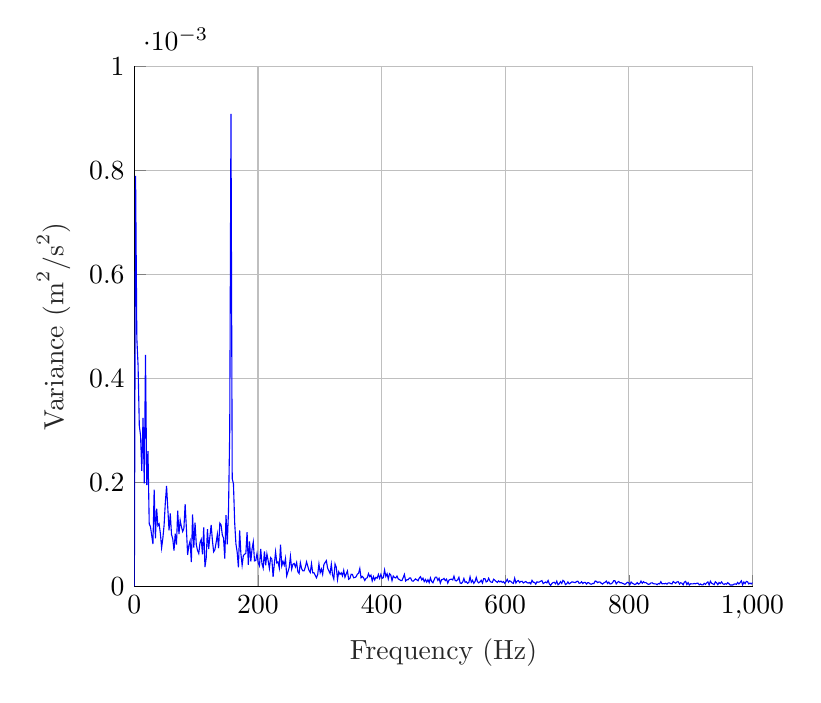
\begin{tikzpicture}

\begin{axis}[%
width=0.951\fwidth,
height=\fheight,
at={(0\fwidth,0\fheight)},
scale only axis,
xmin=0,
xmax=1000,
xlabel style={font=\color{white!15!black}},
xlabel={Frequency (Hz)},
ymin=0,
ymax=0.001,
ylabel style={font=\color{white!15!black}},
ylabel={$\text{Variance (m}^\text{2}\text{/s}^\text{2}\text{)}$},
axis background/.style={fill=white},
axis x line*=bottom,
axis y line*=left,
xmajorgrids,
ymajorgrids
]
\addplot [color=blue, forget plot]
  table[row sep=crcr]{%
0	7.73033949436517e-31\\
2.00400801603206	0.000789460389521223\\
4.00801603206413	0.000477197324178948\\
6.01202404809619	0.000425053536201625\\
8.01603206412826	0.000308731302781442\\
10.0200400801603	0.000290369715741356\\
12.0240480961924	0.000222238216087893\\
14.0280561122244	0.000323945303876248\\
16.0320641282565	0.000198029972857705\\
18.0360721442886	0.000444905616743693\\
20.0400801603206	0.000194741360534741\\
22.0440881763527	0.000259823352234854\\
24.0480961923848	0.000120255112841447\\
26.0521042084168	0.000114849072656891\\
28.0561122244489	9.81658329627821e-05\\
30.060120240481	8.15028585389667e-05\\
32.064128256513	0.00018603606721433\\
34.0681362725451	9.21095334931591e-05\\
36.0721442885772	0.000149482417369553\\
38.0761523046092	0.000116638003656972\\
40.0801603206413	0.000120070231765597\\
42.0841683366733	0.000101804397316884\\
44.0881763527054	7.43100480610313e-05\\
46.0921843687375	9.24270965865502e-05\\
48.0961923847695	0.000117393677641322\\
50.1002004008016	0.000160873838931175\\
52.1042084168337	0.000192981143493375\\
54.1082164328657	0.000150216739269523\\
56.1122244488978	0.000107577299009355\\
58.1162324649299	0.000140077195366813\\
60.1202404809619	9.96168670053149e-05\\
62.124248496994	9.13606768736177e-05\\
64.128256513026	6.88529002466507e-05\\
66.1322645290581	0.00010130130880043\\
68.1362725450902	8.03994678958265e-05\\
70.1402805611222	0.000145714859015586\\
72.1442885771543	0.000100655244035955\\
74.1482965931864	0.00012667637914995\\
76.1523046092184	0.00011460162372702\\
78.1563126252505	0.000105398033525466\\
80.1603206412826	0.000111326971816347\\
82.1643286573146	0.000158256031856355\\
84.1683366733467	0.000112022740041648\\
86.1723446893788	6.03949552007186e-05\\
88.1763527054108	7.86866531801447e-05\\
90.1803607214429	8.7168826579036e-05\\
92.184368737475	4.64245852546354e-05\\
94.188376753507	0.000138146726810315\\
96.1923847695391	7.46241578396251e-05\\
98.1963927855711	0.00012239063764748\\
100.200400801603	8.02190039361078e-05\\
102.204408817635	6.90176877652921e-05\\
104.208416833667	6.31909487755249e-05\\
106.212424849699	8.38580173792474e-05\\
108.216432865731	9.03054079119898e-05\\
110.220440881764	6.14748222886664e-05\\
112.224448897796	0.000113255571245195\\
114.228456913828	3.6989927646902e-05\\
116.23246492986	5.43698357045273e-05\\
118.236472945892	0.000110043747364115\\
120.240480961924	7.1895299295959e-05\\
122.244488977956	9.61922771930644e-05\\
124.248496993988	0.000118171968116645\\
126.25250501002	8.86724911451496e-05\\
128.256513026052	6.65106422187618e-05\\
130.260521042084	7.03153822248777e-05\\
132.264529058116	8.40605249259369e-05\\
134.268537074148	0.000100090484264618\\
136.27254509018	7.33558290671219e-05\\
138.276553106212	0.000121575298753012\\
140.280561122244	0.000118193245630095\\
142.284569138277	9.90791521835578e-05\\
144.288577154309	9.24711109638612e-05\\
146.292585170341	5.33237354550237e-05\\
148.296593186373	0.000136852519276731\\
150.300601202405	8.08885768951026e-05\\
152.304609218437	0.000144641045803664\\
154.308617234469	0.00030007846675525\\
156.312625250501	0.000908545236189398\\
158.316633266533	0.000206996768710833\\
160.320641282565	0.00019717072223189\\
162.324649298597	0.000121989050145497\\
164.328657314629	8.15345569620935e-05\\
166.332665330661	6.59817616147534e-05\\
168.336673346693	3.63731610082001e-05\\
170.340681362725	0.000107608414721268\\
172.344689378758	6.29110834828018e-05\\
174.34869739479	4.05610334320475e-05\\
176.352705410822	5.94542746977593e-05\\
178.356713426854	6.18499410424779e-05\\
180.360721442886	6.34139310000347e-05\\
182.364729458918	0.000104232797298185\\
184.36873747495	4.14843854986565e-05\\
186.372745490982	8.65691312788358e-05\\
188.376753507014	4.78903630407327e-05\\
190.380761523046	7.16091451647836e-05\\
192.384769539078	8.53678405682284e-05\\
194.38877755511	4.89340006360503e-05\\
196.392785571142	4.97680640331037e-05\\
198.396793587174	6.27376772513691e-05\\
200.400801603206	4.50393181870098e-05\\
202.404809619238	3.94857111952775e-05\\
204.408817635271	7.19515721991897e-05\\
206.412825651303	4.37877776086067e-05\\
208.416833667335	3.52241267903507e-05\\
210.420841683367	6.73034610602343e-05\\
212.424849699399	4.05292349084476e-05\\
214.428857715431	6.23287906344995e-05\\
216.432865731463	4.9375121106245e-05\\
218.436873747495	3.44813103480469e-05\\
220.440881763527	5.52105290607725e-05\\
222.444889779559	5.26326815563807e-05\\
224.448897795591	1.82086596488874e-05\\
226.452905811623	4.32986247842451e-05\\
228.456913827655	6.62715621337138e-05\\
230.460921843687	4.4907418965123e-05\\
232.464929859719	4.70039360973566e-05\\
234.468937875751	3.5340732189074e-05\\
236.472945891784	8.01799062305723e-05\\
238.476953907816	3.93258930899951e-05\\
240.480961923848	4.80205237141334e-05\\
242.48496993988	4.08309047674716e-05\\
244.488977955912	5.34977206166746e-05\\
246.492985971944	2.00968828367755e-05\\
248.496993987976	2.80970324210671e-05\\
250.501002004008	3.62998716507292e-05\\
252.50501002004	5.76788616943541e-05\\
254.509018036072	3.31262186659498e-05\\
256.513026052104	4.25067699238326e-05\\
258.517034068136	4.40334775346863e-05\\
260.521042084168	3.74070362971956e-05\\
262.5250501002	4.57376839513042e-05\\
264.529058116232	2.80354399314306e-05\\
266.533066132265	2.48998993582869e-05\\
268.537074148297	4.53845008668962e-05\\
270.541082164329	3.42967710229278e-05\\
272.545090180361	2.97599269042055e-05\\
274.549098196393	2.97929062782659e-05\\
276.553106212425	3.67439914170553e-05\\
278.557114228457	4.71587266088148e-05\\
280.561122244489	3.87559012145459e-05\\
282.565130260521	3.05870939366067e-05\\
284.569138276553	2.6582994093522e-05\\
286.573146292585	4.3585916552445e-05\\
288.577154308617	2.60596030788017e-05\\
290.581162324649	2.61925640792081e-05\\
292.585170340681	2.12040495069082e-05\\
294.589178356713	1.64602459107547e-05\\
296.593186372745	2.26751827211892e-05\\
298.597194388778	4.30712046084884e-05\\
300.60120240481	2.61738411588786e-05\\
302.605210420842	3.30938523654716e-05\\
304.609218436874	2.30756215853302e-05\\
306.613226452906	4.18876673372228e-05\\
308.617234468938	4.59802245474847e-05\\
310.62124248497	4.94688870499771e-05\\
312.625250501002	3.50692279502763e-05\\
314.629258517034	2.97066928597573e-05\\
316.633266533066	2.45336630289745e-05\\
318.637274549098	4.26437820075506e-05\\
320.64128256513	2.15776722691298e-05\\
322.645290581162	1.39479291526418e-05\\
324.649298597194	4.30762623116138e-05\\
326.653306613226	3.68387647206413e-05\\
328.657314629259	1.3154564248057e-05\\
330.661322645291	2.80337687255371e-05\\
332.665330661323	2.31654996494491e-05\\
334.669338677355	2.60722706201826e-05\\
336.673346693387	2.00940580820326e-05\\
338.677354709419	3.08397191192067e-05\\
340.681362725451	1.76522051097235e-05\\
342.685370741483	2.38969580827901e-05\\
344.689378757515	2.95658765992679e-05\\
346.693386773547	1.36293506992759e-05\\
348.697394789579	1.51420530150714e-05\\
350.701402805611	2.3215005508567e-05\\
352.705410821643	2.30160171465513e-05\\
354.709418837675	1.65379580330327e-05\\
356.713426853707	1.69885003805433e-05\\
358.717434869739	1.8482755885007e-05\\
360.721442885772	2.33222262802932e-05\\
362.725450901804	2.50747000488719e-05\\
364.729458917836	3.42714725677784e-05\\
366.733466933868	1.64086877364786e-05\\
368.7374749499	1.9006418249375e-05\\
370.741482965932	1.65081825489174e-05\\
372.745490981964	1.128754395701e-05\\
374.749498997996	1.53600330554115e-05\\
376.753507014028	1.65319155166272e-05\\
378.75751503006	2.44665006519975e-05\\
380.761523046092	1.8742072977736e-05\\
382.765531062124	2.16085261035051e-05\\
384.769539078156	1.04735795816131e-05\\
386.773547094188	1.87161864222571e-05\\
388.77755511022	1.23875349832807e-05\\
390.781563126252	1.73490840992317e-05\\
392.785571142285	1.58231636703342e-05\\
394.789579158317	2.2864019975525e-05\\
396.793587174349	1.53418950088423e-05\\
398.797595190381	2.29952277356298e-05\\
400.801603206413	1.53619480030302e-05\\
402.805611222445	1.68228315376065e-05\\
404.809619238477	3.14421629072224e-05\\
406.813627254509	1.90075129653337e-05\\
408.817635270541	2.42248400772903e-05\\
410.821643286573	1.42247911218015e-05\\
412.825651302605	2.437828147735e-05\\
414.829659318637	2.16834227670185e-05\\
416.833667334669	1.10447196759654e-05\\
418.837675350701	1.98101613311077e-05\\
420.841683366733	1.70332762489214e-05\\
422.845691382766	1.61891727865363e-05\\
424.849699398798	1.97682420554159e-05\\
426.85370741483	1.44045695819494e-05\\
428.857715430862	1.30997027751105e-05\\
430.861723446894	1.11971820469461e-05\\
432.865731462926	1.10947725282203e-05\\
434.869739478958	1.6796472900814e-05\\
436.87374749499	2.29592863119722e-05\\
438.877755511022	1.02548158648226e-05\\
440.881763527054	1.28105866041975e-05\\
442.885771543086	1.26973716719356e-05\\
444.889779559118	1.59321915164122e-05\\
446.89378757515	1.61568685107632e-05\\
448.897795591182	1.08350508528136e-05\\
450.901803607214	9.828595268157e-06\\
452.905811623247	1.19683574704005e-05\\
454.909819639279	1.42393031103468e-05\\
456.913827655311	1.26029001350589e-05\\
458.917835671343	1.07853279989261e-05\\
460.921843687375	1.60359875504741e-05\\
462.925851703407	1.84948774716422e-05\\
464.929859719439	1.24519258339878e-05\\
466.933867735471	1.57333236268542e-05\\
468.937875751503	9.13070993618565e-06\\
470.941883767535	1.32391257141734e-05\\
472.945891783567	8.2645133848288e-06\\
474.949899799599	1.26950495275421e-05\\
476.953907815631	7.23318278992986e-06\\
478.957915831663	1.63192528391295e-05\\
480.961923847695	9.4309655844594e-06\\
482.965931863727	6.80632265991386e-06\\
484.96993987976	1.26441798563012e-05\\
486.973947895792	1.76959310235972e-05\\
488.977955911824	1.76892348890532e-05\\
490.981963927856	1.14840863999741e-05\\
492.985971943888	1.55984161916782e-05\\
494.98997995992	6.32226115009502e-06\\
496.993987975952	1.28038246121979e-05\\
498.997995991984	1.33254379574797e-05\\
501.002004008016	1.52832112117015e-05\\
503.006012024048	1.10288763814428e-05\\
505.01002004008	1.36437987198372e-05\\
507.014028056112	6.27148555929788e-06\\
509.018036072144	1.20662300429994e-05\\
511.022044088176	1.34476332424193e-05\\
513.026052104208	1.37805549757254e-05\\
515.03006012024	1.23547935146404e-05\\
517.034068136273	1.9623092594245e-05\\
519.038076152305	1.11947192252817e-05\\
521.042084168337	1.04696521314059e-05\\
523.046092184369	1.25636078477417e-05\\
525.050100200401	1.74081741998576e-05\\
527.054108216433	6.35814519254982e-06\\
529.058116232465	5.62807265635297e-06\\
531.062124248497	8.21610439924182e-06\\
533.066132264529	1.50175980591918e-05\\
535.070140280561	7.85109035674395e-06\\
537.074148296593	8.816444438517e-06\\
539.078156312625	5.78261348522396e-06\\
541.082164328657	7.37205555233893e-06\\
543.086172344689	1.82979354425625e-05\\
545.090180360721	7.95472062042384e-06\\
547.094188376754	1.16348681664788e-05\\
549.098196392786	5.8966467927905e-06\\
551.102204408818	9.09273148417563e-06\\
553.10621242485	1.71280185063932e-05\\
555.110220440882	9.06722320190997e-06\\
557.114228456914	6.814596331355e-06\\
559.118236472946	8.67222622277829e-06\\
561.122244488978	1.16974950313424e-05\\
563.12625250501	6.36861121091175e-06\\
565.130260521042	1.48761180673437e-05\\
567.134268537074	1.48355140526844e-05\\
569.138276553106	8.49033198582694e-06\\
571.142284569138	9.97533141352473e-06\\
573.14629258517	1.56695349547873e-05\\
575.150300601202	1.0163586402041e-05\\
577.154308617235	8.13196787696348e-06\\
579.158316633267	7.85443738139407e-06\\
581.162324649299	1.36714559611162e-05\\
583.166332665331	1.19620958726531e-05\\
585.170340681363	9.54489578539659e-06\\
587.174348697395	7.57995667795677e-06\\
589.178356713427	1.04057060875794e-05\\
591.182364729459	8.51090115135462e-06\\
593.186372745491	1.00810577331741e-05\\
595.190380761523	7.61927022273169e-06\\
597.194388777555	9.16863335805595e-06\\
599.198396793587	5.78147990386675e-06\\
601.202404809619	9.26167085525013e-06\\
603.206412825651	1.33931910591282e-05\\
605.210420841683	7.87629297344081e-06\\
607.214428857715	1.06848727232494e-05\\
609.218436873747	9.3334588580086e-06\\
611.22244488978	6.70281118467158e-06\\
613.226452905812	5.69641668609057e-06\\
615.230460921844	1.57462438966364e-05\\
617.234468937876	6.54542742382243e-06\\
619.238476953908	9.95784402031918e-06\\
621.24248496994	1.12191681308908e-05\\
623.246492985972	7.27732311436083e-06\\
625.250501002004	9.57753637466972e-06\\
627.254509018036	9.7023149778831e-06\\
629.258517034068	6.460238863165e-06\\
631.2625250501	7.99078066810343e-06\\
633.266533066132	9.29277801377059e-06\\
635.270541082164	7.02908361755636e-06\\
637.274549098196	6.39734219628391e-06\\
639.278557114228	7.36546283489247e-06\\
641.282565130261	4.86630026471822e-06\\
643.286573146293	1.16319069546456e-05\\
645.290581162325	7.87335310967009e-06\\
647.294589178357	7.71931988977348e-06\\
649.298597194389	4.3122476879735e-06\\
651.302605210421	8.71614517709778e-06\\
653.306613226453	7.89045741081801e-06\\
655.310621242485	8.47444761207848e-06\\
657.314629258517	9.96690881350652e-06\\
659.318637274549	1.11233078856992e-05\\
661.322645290581	5.32613616554662e-06\\
663.326653306613	6.82276570992133e-06\\
665.330661322645	8.26143488490662e-06\\
667.334669338677	6.69569944944849e-06\\
669.338677354709	1.1235605124028e-05\\
671.342685370741	4.8266244641051e-06\\
673.346693386773	1.86134455996345e-06\\
675.350701402806	5.36014739260787e-06\\
677.354709418838	7.40733828261044e-06\\
679.35871743487	7.74413894777221e-06\\
681.362725450902	5.01200176085143e-06\\
683.366733466934	9.97730509870779e-06\\
685.370741482966	3.12622474908992e-06\\
687.374749498998	4.99396901163093e-06\\
689.37875751503	9.08799193752845e-06\\
691.382765531062	5.53719315807532e-06\\
693.386773547094	1.15355312829939e-05\\
695.390781563126	9.54212312067055e-06\\
697.394789579158	3.4908260161537e-06\\
699.39879759519	4.82319372663283e-06\\
701.402805611222	8.56379974021921e-06\\
703.406813627255	4.87437477218712e-06\\
705.410821643287	6.35867152776514e-06\\
707.414829659319	8.40861407031583e-06\\
709.418837675351	8.36871156961068e-06\\
711.422845691383	7.66238036097647e-06\\
713.426853707415	7.17548289105782e-06\\
715.430861723447	9.42479723509089e-06\\
717.434869739479	9.91304959792542e-06\\
719.438877755511	5.9364093518101e-06\\
721.442885771543	6.25298797766602e-06\\
723.446893787575	8.88759800930205e-06\\
725.450901803607	5.46876387965262e-06\\
727.454909819639	7.41153713543619e-06\\
729.458917835671	7.59388127648185e-06\\
731.462925851703	4.41089225400736e-06\\
733.466933867736	7.16291708220795e-06\\
735.470941883768	6.80370524391558e-06\\
737.4749498998	4.61040934405302e-06\\
739.478957915832	4.09248775070101e-06\\
741.482965931864	5.65421611867832e-06\\
743.486973947896	5.26108027805286e-06\\
745.490981963928	1.03345499780691e-05\\
747.49498997996	9.48350073977794e-06\\
749.498997995992	7.11903680040851e-06\\
751.503006012024	8.36492085693384e-06\\
753.507014028056	8.20951653346917e-06\\
755.511022044088	5.67786694810645e-06\\
757.51503006012	4.36361603808858e-06\\
759.519038076152	6.74306164223293e-06\\
761.523046092184	7.73412777719714e-06\\
763.527054108216	1.00361784608525e-05\\
765.531062124248	5.47216458758696e-06\\
767.535070140281	8.01360787469499e-06\\
769.539078156313	4.42706754869714e-06\\
771.543086172345	5.11353811183089e-06\\
773.547094188377	6.86357237197911e-06\\
775.551102204409	1.09579047626253e-05\\
777.555110220441	1.06746616971011e-05\\
779.559118236473	4.73067584499269e-06\\
781.563126252505	7.72932901185093e-06\\
783.567134268537	9.36475094196777e-06\\
785.571142284569	6.72858129990758e-06\\
787.575150300601	7.148731271046e-06\\
789.579158316633	5.87762527975675e-06\\
791.583166332665	5.04181483097194e-06\\
793.587174348697	3.8182652481529e-06\\
795.591182364729	5.40151853800462e-06\\
797.595190380762	7.7507004331823e-06\\
799.599198396794	6.84240452740476e-06\\
801.603206412826	3.28238210333565e-06\\
803.607214428858	8.3183385372571e-06\\
805.61122244489	5.82865191813924e-06\\
807.615230460922	4.79879388547051e-06\\
809.619238476954	3.38579375196902e-06\\
811.623246492986	4.65930348847307e-06\\
813.627254509018	6.98583905381384e-06\\
815.63126252505	4.38843567421742e-06\\
817.635270541082	5.66331137066874e-06\\
819.639278557114	1.0060712731066e-05\\
821.643286573146	5.95990039380616e-06\\
823.647294589178	8.93696911738855e-06\\
825.65130260521	7.01422835325668e-06\\
827.655310621243	7.2667860145611e-06\\
829.659318637275	5.23056343803039e-06\\
831.663326653307	3.77731377090095e-06\\
833.667334669339	4.45114052655796e-06\\
835.671342685371	6.55421874477506e-06\\
837.675350701403	6.82906719191064e-06\\
839.679358717435	5.20476257606069e-06\\
841.683366733467	4.82350843995292e-06\\
843.687374749499	4.72898599702169e-06\\
845.691382765531	3.1749666002953e-06\\
847.695390781563	5.41446076729101e-06\\
849.699398797595	4.67506785986846e-06\\
851.703406813627	8.98030536346748e-06\\
853.707414829659	4.81932099620709e-06\\
855.711422845691	5.27652818415778e-06\\
857.715430861723	4.90240721520228e-06\\
859.719438877755	5.86649933115119e-06\\
861.723446893788	4.25109230352562e-06\\
863.72745490982	6.66869721930127e-06\\
865.731462925852	6.64586701529853e-06\\
867.735470941884	5.23928375943846e-06\\
869.739478957916	4.667233718657e-06\\
871.743486973948	9.26302247165903e-06\\
873.74749498998	7.37505342209734e-06\\
875.751503006012	5.9444995978887e-06\\
877.755511022044	8.37639259559014e-06\\
879.759519038076	9.03592836413124e-06\\
881.763527054108	4.37626324566635e-06\\
883.76753507014	6.92823531065501e-06\\
885.771543086172	5.97356517178297e-06\\
887.775551102204	2.98513377964991e-06\\
889.779559118236	8.18036174853934e-06\\
891.783567134269	9.57305077162671e-06\\
893.787575150301	3.50815564028152e-06\\
895.791583166333	7.17172167690305e-06\\
897.795591182365	2.6405950094716e-06\\
899.799599198397	5.04716414686626e-06\\
901.803607214429	4.78119937005335e-06\\
903.807615230461	4.716392561841e-06\\
905.811623246493	5.55528318813793e-06\\
907.815631262525	4.8314719025891e-06\\
909.819639278557	5.95635713701505e-06\\
911.823647294589	5.97572376676137e-06\\
913.827655310621	3.03980918551666e-06\\
915.831663326653	4.66552124303148e-06\\
917.835671342685	2.9805550650226e-06\\
919.839679358717	2.89354509358309e-06\\
921.843687374749	5.78696685290324e-06\\
923.847695390782	3.87260720301145e-06\\
925.851703406814	6.69598765845818e-06\\
927.855711422846	8.52465883300403e-06\\
929.859719438878	2.68938408601591e-06\\
931.86372745491	9.80993060519215e-06\\
933.867735470942	5.91947722980712e-06\\
935.871743486974	4.85922986773526e-06\\
937.875751503006	3.29516896290309e-06\\
939.879759519038	8.70976114063155e-06\\
941.88376753507	6.86514038059465e-06\\
943.887775551102	3.2274646062745e-06\\
945.891783567134	7.29926375769909e-06\\
947.895791583166	5.42149273042046e-06\\
949.899799599198	8.60322901068689e-06\\
951.90380761523	4.99599537862958e-06\\
953.907815631263	3.77138367310521e-06\\
955.911823647295	5.14085836832939e-06\\
957.915831663327	4.17651134756703e-06\\
959.919839679359	7.11629970481619e-06\\
961.923847695391	5.14646832929149e-06\\
963.927855711423	2.54412118927411e-06\\
965.931863727455	2.55649407018669e-06\\
967.935871743487	2.51731858619676e-06\\
969.939879759519	4.25839618265826e-06\\
971.943887775551	4.76819827240278e-06\\
973.947895791583	3.89408244133317e-06\\
975.951903807615	7.50801551468693e-06\\
977.955911823647	4.70911775411267e-06\\
979.959919839679	7.11082107755246e-06\\
981.963927855711	1.06188277822257e-05\\
983.967935871744	2.72112647342951e-06\\
985.971943887776	8.30969484766394e-06\\
987.975951903808	5.153771451331e-06\\
989.97995991984	9.45379977797844e-06\\
991.983967935872	8.68861449005863e-06\\
993.987975951904	4.63072185725119e-06\\
995.991983967936	6.18785169507163e-06\\
997.995991983968	4.62762459717101e-06\\
1000	7.16716397726108e-06\\
};
\end{axis}
\end{tikzpicture}%
    \caption{Velocity spectra when the hot wire anemometer was inline with the top of the cylinder.}
    \label{fig:freq3}
\end{figure}
\vspace{0.5cm}
\begin{figure}[H]
    \centering
    % This file was created by matlab2tikz.
%
%The latest updates can be retrieved from
%  http://www.mathworks.com/matlabcentral/fileexchange/22022-matlab2tikz-matlab2tikz
%where you can also make suggestions and rate matlab2tikz.
%
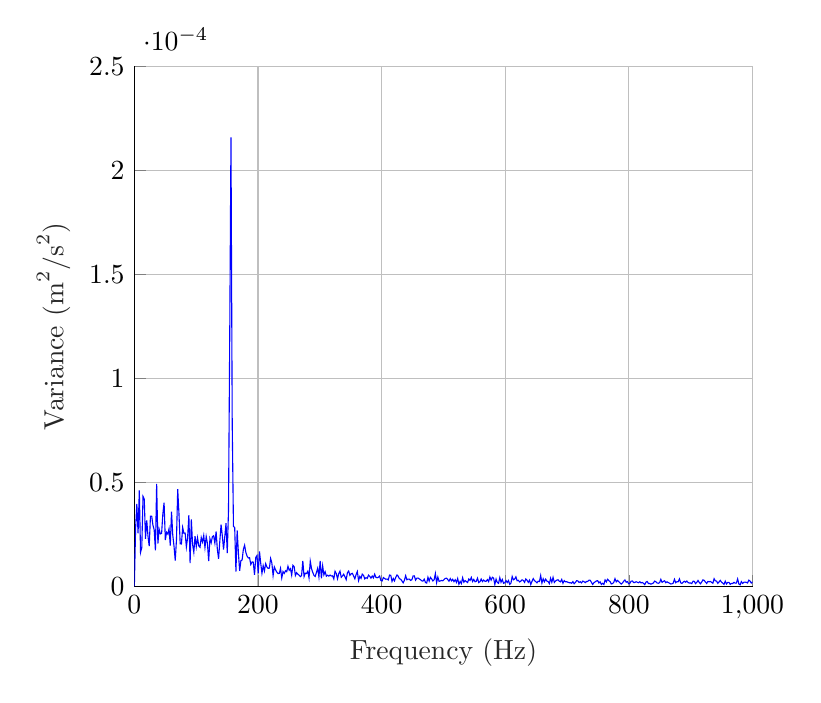
\begin{tikzpicture}

\begin{axis}[%
width=0.951\fwidth,
height=\fheight,
at={(0\fwidth,0\fheight)},
scale only axis,
xmin=0,
xmax=1000,
xlabel style={font=\color{white!15!black}},
xlabel={Frequency (Hz)},
ymin=0,
ymax=0.00025,
ylabel style={font=\color{white!15!black}},
ylabel={$\text{Variance (m}^\text{2}\text{/s}^\text{2}\text{)}$},
axis background/.style={fill=white},
axis x line*=bottom,
axis y line*=left,
xmajorgrids,
ymajorgrids
]
\addplot [color=blue, forget plot]
  table[row sep=crcr]{%
0	1.06956155722712e-30\\
2.00400801603206	2.79002842990907e-05\\
4.00801603206413	3.96097633465834e-05\\
6.01202404809619	2.55043261177493e-05\\
8.01603206412826	4.61778670735352e-05\\
10.0200400801603	1.62690468977124e-05\\
12.0240480961924	1.86335300988678e-05\\
14.0280561122244	4.32318604853325e-05\\
16.0320641282565	4.19166206505963e-05\\
18.0360721442886	2.28681563663269e-05\\
20.0400801603206	3.17063307058159e-05\\
22.0440881763527	2.41639720803978e-05\\
24.0480961923848	1.93166447911753e-05\\
26.0521042084168	3.37624278227763e-05\\
28.0561122244489	3.37828482056573e-05\\
30.060120240481	2.94001687127763e-05\\
32.064128256513	2.72178201500007e-05\\
34.0681362725451	1.72716106146422e-05\\
36.0721442885772	4.92303148823583e-05\\
38.0761523046092	2.05628206217393e-05\\
40.0801603206413	2.74804929808399e-05\\
42.0841683366733	2.52280838746124e-05\\
44.0881763527054	2.54770814500535e-05\\
46.0921843687375	3.47873350909514e-05\\
48.0961923847695	4.0265816168591e-05\\
50.1002004008016	2.22201962349941e-05\\
52.1042084168337	2.59892283843544e-05\\
54.1082164328657	2.5143373406651e-05\\
56.1122244488978	2.76711640055986e-05\\
58.1162324649299	1.95613017086139e-05\\
60.1202404809619	3.59024298437653e-05\\
62.124248496994	2.47383183229815e-05\\
64.128256513026	1.9405770726171e-05\\
66.1322645290581	1.24284822344416e-05\\
68.1362725450902	2.23435351710562e-05\\
70.1402805611222	4.67276374327979e-05\\
72.1442885771543	3.5181541798417e-05\\
74.1482965931864	2.04354952099042e-05\\
76.1523046092184	2.03709153480391e-05\\
78.1563126252505	2.83028156002955e-05\\
80.1603206412826	2.55463855798805e-05\\
82.1643286573146	2.56109735780645e-05\\
84.1683366733467	1.89285580830902e-05\\
86.1723446893788	2.34625279668094e-05\\
88.1763527054108	3.4207698484594e-05\\
90.1803607214429	1.11888402034038e-05\\
92.184368737475	3.21928805479732e-05\\
94.188376753507	2.01378299492548e-05\\
96.1923847695391	1.63969621614684e-05\\
98.1963927855711	2.41296039919898e-05\\
100.200400801603	1.90786523523118e-05\\
102.204408817635	2.33209194667847e-05\\
104.208416833667	1.95034534203438e-05\\
106.212424849699	1.87823362904317e-05\\
108.216432865731	2.34782862443169e-05\\
110.220440881764	2.13370516857386e-05\\
112.224448897796	2.44482522932589e-05\\
114.228456913828	1.86365531538259e-05\\
116.23246492986	2.39548035938856e-05\\
118.236472945892	2.05447605598407e-05\\
120.240480961924	1.21507889697189e-05\\
122.244488977956	2.29143069456296e-05\\
124.248496993988	2.09005114808357e-05\\
126.25250501002	2.39140634541448e-05\\
128.256513026052	2.42978461756479e-05\\
130.260521042084	2.07731106459725e-05\\
132.264529058116	2.63707097499859e-05\\
134.268537074148	1.78206110629323e-05\\
136.27254509018	1.32426033690861e-05\\
138.276553106212	2.18093318220857e-05\\
140.280561122244	2.97057422873419e-05\\
142.284569138277	2.44424180315704e-05\\
144.288577154309	1.77370212092435e-05\\
146.292585170341	2.38576845429127e-05\\
148.296593186373	3.03575816960738e-05\\
150.300601202405	1.59955706948066e-05\\
152.304609218437	3.64183083974016e-05\\
154.308617234469	0.000120614480183573\\
156.312625250501	0.000215873635566948\\
158.316633266533	7.84879749304883e-05\\
160.320641282565	2.88218556760604e-05\\
162.324649298597	2.82463498279982e-05\\
164.328657314629	7.12608826436887e-06\\
166.332665330661	2.69055001359479e-05\\
168.336673346693	1.59389352306358e-05\\
170.340681362725	7.45139478576233e-06\\
172.344689378758	1.23908787158559e-05\\
174.34869739479	1.26631631720164e-05\\
176.352705410822	1.78272478179015e-05\\
178.356713426854	1.97585043731262e-05\\
180.360721442886	1.63116281305506e-05\\
182.364729458918	1.4525541306177e-05\\
184.36873747495	1.36413361932612e-05\\
186.372745490982	1.37532771192e-05\\
188.376753507014	1.05390395701397e-05\\
190.380761523046	1.17276640935581e-05\\
192.384769539078	1.16583979941971e-05\\
194.38877755511	5.52627577139883e-06\\
196.392785571142	1.38755729702626e-05\\
198.396793587174	1.48286570854015e-05\\
200.400801603206	6.28210698280652e-06\\
202.404809619238	1.68437223242438e-05\\
204.408817635271	1.11636235112429e-05\\
206.412825651303	6.282360985457e-06\\
208.416833667335	9.92447628023483e-06\\
210.420841683367	7.42134769343557e-06\\
212.424849699399	1.09081401401721e-05\\
214.428857715431	9.32770772978902e-06\\
216.432865731463	8.61228258824247e-06\\
218.436873747495	8.77736966415782e-06\\
220.440881763527	1.34021879474301e-05\\
222.444889779559	1.1252479982503e-05\\
224.448897795591	5.15642085350804e-06\\
226.452905811623	9.33602926968332e-06\\
228.456913827655	7.90274226916947e-06\\
230.460921843687	6.86587007571418e-06\\
232.464929859719	6.14110709999506e-06\\
234.468937875751	6.20981671101964e-06\\
236.472945891784	8.63953577048601e-06\\
238.476953907816	4.0191565257541e-06\\
240.480961923848	7.10545719816408e-06\\
242.48496993988	6.22024271522449e-06\\
244.488977955912	7.49468774673133e-06\\
246.492985971944	7.05593217670373e-06\\
248.496993987976	9.67090544891434e-06\\
250.501002004008	7.74409545677429e-06\\
252.50501002004	8.47061494192062e-06\\
254.509018036072	5.40699324245527e-06\\
256.513026052104	1.01150896277229e-05\\
258.517034068136	9.53353036814547e-06\\
260.521042084168	5.21010630691459e-06\\
262.5250501002	6.56667670467937e-06\\
264.529058116232	5.84571161695057e-06\\
266.533066132265	5.3755036245567e-06\\
268.537074148297	4.6783398620355e-06\\
270.541082164329	5.22265270357122e-06\\
272.545090180361	1.22507542859999e-05\\
274.549098196393	4.69618821953591e-06\\
276.553106212425	6.33266228447408e-06\\
278.557114228457	6.17661697237688e-06\\
280.561122244489	7.25791089223237e-06\\
282.565130260521	4.05474766246182e-06\\
284.569138276553	1.20985582953302e-05\\
286.573146292585	8.53782947072016e-06\\
288.577154308617	6.76576495417072e-06\\
290.581162324649	5.2723918661556e-06\\
292.585170340681	4.76944763695386e-06\\
294.589178356713	6.70369087358413e-06\\
296.593186372745	8.73143350123109e-06\\
298.597194388778	4.53413328171529e-06\\
300.60120240481	1.2201203956553e-05\\
302.605210420842	3.86940027625843e-06\\
304.609218436874	9.85825832454381e-06\\
306.613226452906	5.52941693226043e-06\\
308.617234468938	7.02027365248701e-06\\
310.62124248497	4.89538938755413e-06\\
312.625250501002	5.36655691031281e-06\\
314.629258517034	4.93295078267524e-06\\
316.633266533066	5.41108981191289e-06\\
318.637274549098	4.97701690577189e-06\\
320.64128256513	5.06310991378262e-06\\
322.645290581162	3.55550212508909e-06\\
324.649298597194	7.23506954806386e-06\\
326.653306613226	6.18515892282291e-06\\
328.657314629259	3.61649120246706e-06\\
330.661322645291	6.07750506979145e-06\\
332.665330661323	7.31246470233379e-06\\
334.669338677355	4.37163302268518e-06\\
336.673346693387	5.01937619488405e-06\\
338.677354709419	5.84441266865415e-06\\
340.681362725451	4.60714897661545e-06\\
342.685370741483	3.22477210089098e-06\\
344.689378757515	6.5365292835654e-06\\
346.693386773547	7.32823894075181e-06\\
348.697394789579	5.29731332008979e-06\\
350.701402805611	6.0393450721916e-06\\
352.705410821643	6.24354471291267e-06\\
354.709418837675	4.95529476002703e-06\\
356.713426853707	3.62321279454651e-06\\
358.717434869739	5.6957147532624e-06\\
360.721442885772	7.15390563265923e-06\\
362.725450901804	2.74784474937249e-06\\
364.729458917836	4.75361150859468e-06\\
366.733466933868	3.85141072508632e-06\\
368.7374749499	5.88773973745756e-06\\
370.741482965932	5.30165001241336e-06\\
372.745490981964	3.59699346245402e-06\\
374.749498997996	4.17757676755042e-06\\
376.753507014028	3.83654177814909e-06\\
378.75751503006	5.39031613936895e-06\\
380.761523046092	4.81208381686074e-06\\
382.765531062124	3.95717032407982e-06\\
384.769539078156	4.96954357869323e-06\\
386.773547094188	4.05611403751186e-06\\
388.77755511022	5.85410732350827e-06\\
390.781563126252	4.31511754095613e-06\\
392.785571142285	4.13262979447265e-06\\
394.789579158317	4.35330955959751e-06\\
396.793587174349	4.94646908096586e-06\\
398.797595190381	2.81283967813575e-06\\
400.801603206413	2.57827805693536e-06\\
402.805611222445	4.22959707604579e-06\\
404.809619238477	3.81900544060491e-06\\
406.813627254509	3.41812151169035e-06\\
408.817635270541	3.51283861598502e-06\\
410.821643286573	3.11146405560783e-06\\
412.825651302605	5.42054222412434e-06\\
414.829659318637	5.28115325325118e-06\\
416.833667334669	2.35604434881636e-06\\
418.837675350701	3.7852372869359e-06\\
420.841683366733	2.6500391648741e-06\\
422.845691382766	4.31996035975788e-06\\
424.849699398798	5.45306937697007e-06\\
426.85370741483	4.86723752001535e-06\\
428.857715430862	3.66968609813839e-06\\
430.861723446894	3.41769652087457e-06\\
432.865731462926	2.60398177484445e-06\\
434.869739478958	1.68846432804164e-06\\
436.87374749499	2.92497726483236e-06\\
438.877755511022	5.14318969362684e-06\\
440.881763527054	3.17579632182844e-06\\
442.885771543086	3.48808925837911e-06\\
444.889779559118	3.48078407360738e-06\\
446.89378757515	2.85962311881363e-06\\
448.897795591182	3.14938467336533e-06\\
450.901803607214	4.98018426603652e-06\\
452.905811623247	5.05126221078373e-06\\
454.909819639279	2.99033388624216e-06\\
456.913827655311	3.93122529109401e-06\\
458.917835671343	3.99126216099662e-06\\
460.921843687375	3.60092388392431e-06\\
462.925851703407	3.21042093539646e-06\\
464.929859719439	2.63661263466871e-06\\
466.933867735471	2.51822889762319e-06\\
468.937875751503	3.4575321810601e-06\\
470.941883767535	1.84168445808506e-06\\
472.945891783567	1.59016630410845e-06\\
474.949899799599	4.37924402710089e-06\\
476.953907815631	2.51986752049873e-06\\
478.957915831663	4.3142313461486e-06\\
480.961923847695	3.56578290675755e-06\\
482.965931863727	2.56633984811203e-06\\
484.96993987976	3.18161112632509e-06\\
486.973947895792	6.13133864027375e-06\\
488.977955911824	1.77783279398026e-06\\
490.981963927856	4.46800526227096e-06\\
492.985971943888	2.40814560015497e-06\\
494.98997995992	2.59758984381261e-06\\
496.993987975952	2.84723782487894e-06\\
498.997995991984	2.65793863155441e-06\\
501.002004008016	3.27504027572989e-06\\
503.006012024048	3.80588893848775e-06\\
505.01002004008	3.94636150426054e-06\\
507.014028056112	3.27590481873127e-06\\
509.018036072144	2.47587069556399e-06\\
511.022044088176	3.7572185438997e-06\\
513.026052104208	2.64620529895816e-06\\
515.03006012024	3.39526742305428e-06\\
517.034068136273	2.25398787335141e-06\\
519.038076152305	3.20733262365946e-06\\
521.042084168337	1.91755633304936e-06\\
523.046092184369	3.78058327779665e-06\\
525.050100200401	1.0155256469236e-06\\
527.054108216433	2.36427528595169e-06\\
529.058116232465	1.33710089674233e-06\\
531.062124248497	4.14316234585065e-06\\
533.066132264529	1.99214446280942e-06\\
535.070140280561	2.78118329497289e-06\\
537.074148296593	2.28675151373378e-06\\
539.078156312625	1.83844211076503e-06\\
541.082164328657	3.55263743336925e-06\\
543.086172344689	2.84701083363456e-06\\
545.090180360721	4.28371062076511e-06\\
547.094188376754	2.31151737887306e-06\\
549.098196392786	3.33376357343675e-06\\
551.102204408818	2.20678846672215e-06\\
553.10621242485	2.43770332808109e-06\\
555.110220440882	3.94964315996596e-06\\
557.114228456914	1.80960223404093e-06\\
559.118236472946	2.27970342266117e-06\\
561.122244488978	3.51410986181644e-06\\
563.12625250501	2.30372854211422e-06\\
565.130260521042	3.03902341022219e-06\\
567.134268537074	2.47873938406042e-06\\
569.138276553106	2.45554216271495e-06\\
571.142284569138	3.2725528894e-06\\
573.14629258517	2.26383811652163e-06\\
575.150300601202	4.49850920564502e-06\\
577.154308617235	2.98557158001246e-06\\
579.158316633267	4.35978285630093e-06\\
581.162324649299	3.9684334293403e-06\\
583.166332665331	9.29688413234399e-07\\
585.170340681363	3.50324626473809e-06\\
587.174348697395	1.88125867541242e-06\\
589.178356713427	1.47085606053046e-06\\
591.182364729459	4.18425932867152e-06\\
593.186372745491	1.98371751653223e-06\\
595.190380761523	3.28341902787335e-06\\
597.194388777555	1.46691971050476e-06\\
599.198396793587	1.6775999630748e-06\\
601.202404809619	2.76744259951867e-06\\
603.206412825651	1.84221805990723e-06\\
605.210420841683	2.81146690249293e-06\\
607.214428857715	9.67903169768774e-07\\
609.218436873747	1.54584181994942e-06\\
611.22244488978	4.72627334539949e-06\\
613.226452905812	3.15716713217566e-06\\
615.230460921844	3.49467396206063e-06\\
617.234468937876	4.57235313053545e-06\\
619.238476953908	2.68096918519879e-06\\
621.24248496994	2.87661475930621e-06\\
623.246492985972	2.12718344949089e-06\\
625.250501002004	2.51648297754777e-06\\
627.254509018036	3.12381017579678e-06\\
629.258517034068	2.86214934659614e-06\\
631.2625250501	1.94096983878533e-06\\
633.266533066132	3.54702950937518e-06\\
635.270541082164	2.91462735584598e-06\\
637.274549098196	1.95671373943322e-06\\
639.278557114228	2.99046866791158e-06\\
641.282565130261	8.89088252709724e-07\\
643.286573146293	2.4299658809906e-06\\
645.290581162325	3.72045776499685e-06\\
647.294589178357	2.75200933221476e-06\\
649.298597194389	2.3130496995954e-06\\
651.302605210421	1.6955231811983e-06\\
653.306613226453	2.46945514778838e-06\\
655.310621242485	2.32670782215213e-06\\
657.314629258517	5.17243421232219e-06\\
659.318637274549	1.5663654982936e-06\\
661.322645290581	3.61146623208712e-06\\
663.326653306613	2.17403857954305e-06\\
665.330661322645	3.45695126732981e-06\\
667.334669338677	2.53844080553267e-06\\
669.338677354709	2.29840969872636e-06\\
671.342685370741	1.30128038014313e-06\\
673.346693386773	3.8816778517212e-06\\
675.350701402806	1.99207783699372e-06\\
677.354709418838	4.28369259868131e-06\\
679.35871743487	1.88713396445097e-06\\
681.362725450902	2.55308498498955e-06\\
683.366733466934	2.99296007530885e-06\\
685.370741482966	3.15680012904099e-06\\
687.374749498998	2.45377949557832e-06\\
689.37875751503	2.18910955516844e-06\\
691.382765531062	3.31629282592723e-06\\
693.386773547094	1.46648955948284e-06\\
695.390781563126	2.72966672400447e-06\\
697.394789579158	2.14467829138248e-06\\
699.39879759519	2.24785249715077e-06\\
701.402805611222	1.94178869387044e-06\\
703.406813627255	1.75447304269184e-06\\
705.410821643287	1.75032313934225e-06\\
707.414829659319	1.47798252072155e-06\\
709.418837675351	2.27378756248163e-06\\
711.422845691383	1.27301200462978e-06\\
713.426853707415	1.82284210015999e-06\\
715.430861723447	2.7430754914969e-06\\
717.434869739479	2.60503294087308e-06\\
719.438877755511	1.90098909903819e-06\\
721.442885771543	2.19450997291395e-06\\
723.446893787575	1.66769896472148e-06\\
725.450901803607	2.52147502590227e-06\\
727.454909819639	2.27148415320543e-06\\
729.458917835671	1.77548574666922e-06\\
731.462925851703	2.32532263809684e-06\\
733.466933867736	2.36394338762713e-06\\
735.470941883768	3.00623702812124e-06\\
737.4749498998	2.91394056163532e-06\\
739.478957915832	1.91301258488048e-06\\
741.482965931864	9.17689598678396e-07\\
743.486973947896	1.76269769464262e-06\\
745.490981963928	2.16384938601984e-06\\
747.49498997996	2.60155058259229e-06\\
749.498997995992	2.74487049877821e-06\\
751.503006012024	1.63882047875272e-06\\
753.507014028056	2.17162724865186e-06\\
755.511022044088	9.05076504921742e-07\\
757.51503006012	1.46171305802042e-06\\
759.519038076152	8.6489092454589e-07\\
761.523046092184	3.10264956535943e-06\\
763.527054108216	2.156755868496e-06\\
765.531062124248	3.39630045705862e-06\\
767.535070140281	2.75902455943342e-06\\
769.539078156313	2.2927763442557e-06\\
771.543086172345	1.14174087565119e-06\\
773.547094188377	1.35882029910246e-06\\
775.551102204409	1.9043986298904e-06\\
777.555110220441	3.69190552064916e-06\\
779.559118236473	2.17268186096081e-06\\
781.563126252505	2.85436833938823e-06\\
783.567134268537	2.30026194869279e-06\\
785.571142284569	1.73021014840058e-06\\
787.575150300601	1.09996372734306e-06\\
789.579158316633	1.60650975328802e-06\\
791.583166332665	2.44709838878339e-06\\
793.587174348697	3.10386344957462e-06\\
795.591182364729	1.99761237573083e-06\\
797.595190380762	2.24734134077149e-06\\
799.599198396794	1.30239964033449e-06\\
801.603206412826	1.48371031347184e-06\\
803.607214428858	2.43940423635586e-06\\
805.61122244489	2.62009170294503e-06\\
807.615230460922	1.8371597053028e-06\\
809.619238476954	1.87325204862145e-06\\
811.623246492986	2.20886168048218e-06\\
813.627254509018	1.99752768217396e-06\\
815.63126252505	1.72424862922668e-06\\
817.635270541082	2.21613494873008e-06\\
819.639278557114	1.65657755851392e-06\\
821.643286573146	1.90470771528106e-06\\
823.647294589178	1.45901996536246e-06\\
825.65130260521	8.40833640880569e-07\\
827.655310621243	2.05509606121167e-06\\
829.659318637275	2.34079407755941e-06\\
831.663326653307	1.33296402034937e-06\\
833.667334669339	1.40573329460816e-06\\
835.671342685371	1.05426129475574e-06\\
837.675350701403	1.310167166468e-06\\
839.679358717435	1.63466292912847e-06\\
841.683366733467	2.51447129587916e-06\\
843.687374749499	2.22127901988065e-06\\
845.691382765531	1.58547994018037e-06\\
847.695390781563	1.49668840094472e-06\\
849.699398797595	1.76615194954339e-06\\
851.703406813627	3.37293145702175e-06\\
853.707414829659	1.94523269040668e-06\\
855.711422845691	2.35366427145618e-06\\
857.715430861723	2.67092284411621e-06\\
859.719438877755	1.74793734570746e-06\\
861.723446893788	2.17744618171168e-06\\
863.72745490982	1.79792247270524e-06\\
865.731462925852	1.55929646047749e-06\\
867.735470941884	1.1309097198913e-06\\
869.739478957916	1.23046015588263e-06\\
871.743486973948	1.56938719586804e-06\\
873.74749498998	3.38407713719078e-06\\
875.751503006012	1.77703797794583e-06\\
877.755511022044	2.25119379735103e-06\\
879.759519038076	2.20794555355979e-06\\
881.763527054108	3.55472401654177e-06\\
883.76753507014	1.72700256243481e-06\\
885.771543086172	1.40518473454829e-06\\
887.775551102204	2.00158943872007e-06\\
889.779559118236	2.45928837014834e-06\\
891.783567134269	1.96817666097281e-06\\
893.787575150301	2.54989764620326e-06\\
895.791583166333	1.81923756480506e-06\\
897.795591182365	1.55899585017799e-06\\
899.799599198397	1.63442767219526e-06\\
901.803607214429	1.33769887159237e-06\\
903.807615230461	2.47511306265683e-06\\
905.811623246493	2.41738035404246e-06\\
907.815631262525	1.3151116691328e-06\\
909.819639278557	1.8766224858903e-06\\
911.823647294589	2.81135467418912e-06\\
913.827655310621	1.90136988308282e-06\\
915.831663326653	1.22430105019255e-06\\
917.835671342685	2.10114711726708e-06\\
919.839679358717	3.10915378342925e-06\\
921.843687374749	2.88919387355808e-06\\
923.847695390782	2.06975764620422e-06\\
925.851703406814	1.41625082593522e-06\\
927.855711422846	2.35304216450119e-06\\
929.859719438878	2.168156527467e-06\\
931.86372745491	2.36649002145233e-06\\
933.867735470942	1.90180738251888e-06\\
935.871743486974	1.52095760216088e-06\\
937.875751503006	3.67553880366156e-06\\
939.879759519038	2.64500713440701e-06\\
941.88376753507	2.52493073125248e-06\\
943.887775551102	1.44639571372529e-06\\
945.891783567134	2.11713531720093e-06\\
947.895791583166	2.88874746626944e-06\\
949.899799599198	2.00230853544723e-06\\
951.90380761523	1.52931871919299e-06\\
953.907815631263	9.61011123696457e-07\\
955.911823647295	2.50251374019687e-06\\
957.915831663327	1.16455243086156e-06\\
959.919839679359	1.94260410373364e-06\\
961.923847695391	1.94252689062547e-06\\
963.927855711423	9.55987387092119e-07\\
965.931863727455	1.42018732420722e-06\\
967.935871743487	1.37450485882158e-06\\
969.939879759519	1.91782491428377e-06\\
971.943887775551	1.51778719375472e-06\\
973.947895791583	1.59347433874256e-06\\
975.951903807615	3.56776320706494e-06\\
977.955911823647	1.11715535399884e-06\\
979.959919839679	7.26838531308765e-07\\
981.963927855711	2.26012120003726e-06\\
983.967935871744	1.42394476786536e-06\\
985.971943887776	1.96878230615663e-06\\
987.975951903808	2.04211384766371e-06\\
989.97995991984	1.91369725905e-06\\
991.983967935872	1.60800062176521e-06\\
993.987975951904	2.97759514295532e-06\\
995.991983967936	2.55251129772237e-06\\
997.995991983968	1.62136528828907e-06\\
1000	2.11226408638334e-06\\
};
\end{axis}
\end{tikzpicture}%
    \caption{Velocity spectra when the hot wire anemometer was in the flow wake region.}
    \label{fig:freq4}
\end{figure}
\vspace{-1.5cm}
\begin{figure}[H]
    \centering
    % This file was created by matlab2tikz.
%
%The latest updates can be retrieved from
%  http://www.mathworks.com/matlabcentral/fileexchange/22022-matlab2tikz-matlab2tikz
%where you can also make suggestions and rate matlab2tikz.
%
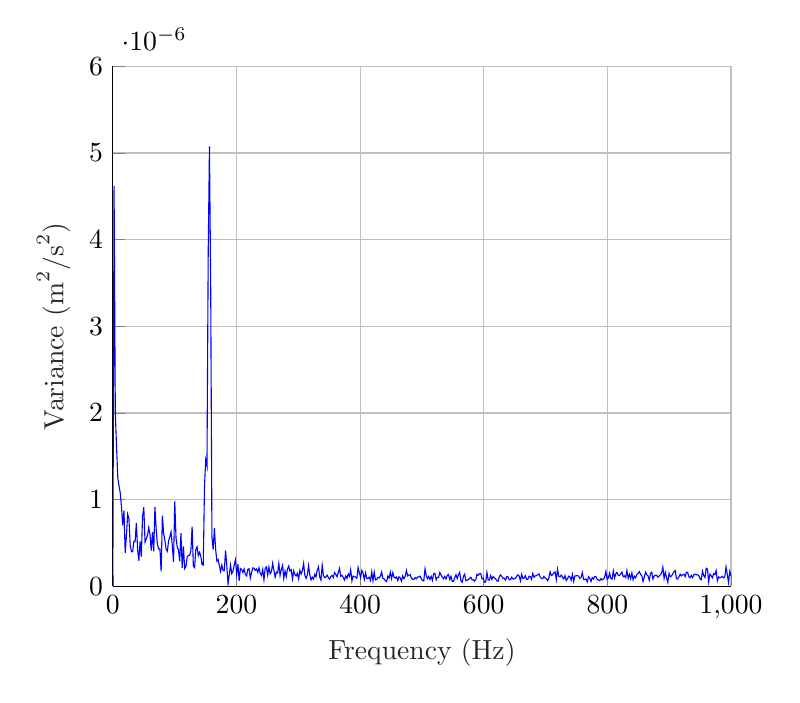
\begin{tikzpicture}

\begin{axis}[%
width=0.951\fwidth,
height=\fheight,
at={(0\fwidth,0\fheight)},
scale only axis,
xmin=0,
xmax=1000,
xlabel style={font=\color{white!15!black}},
xlabel={Frequency (Hz)},
ymin=0,
ymax=6e-06,
ylabel style={font=\color{white!15!black}},
ylabel={$\text{Variance (m}^\text{2}\text{/s}^\text{2}\text{)}$},
axis background/.style={fill=white},
axis x line*=bottom,
axis y line*=left,
xmajorgrids,
ymajorgrids
]
\addplot [color=blue, forget plot]
  table[row sep=crcr]{%
0	7.06896363902376e-31\\
2.00400801603206	4.62075338270973e-06\\
4.00801603206413	2.00148448041867e-06\\
6.01202404809619	1.61065627990101e-06\\
8.01603206412826	1.25607613183047e-06\\
10.0200400801603	1.15722835193769e-06\\
12.0240480961924	1.07551883581034e-06\\
14.0280561122244	9.16163413915246e-07\\
16.0320641282565	7.03397547988298e-07\\
18.0360721442886	8.7276495641411e-07\\
20.0400801603206	3.86968842570606e-07\\
22.0440881763527	5.89908263314714e-07\\
24.0480961923848	8.31081615847116e-07\\
26.0521042084168	7.77565394404703e-07\\
28.0561122244489	4.77871282719007e-07\\
30.060120240481	4.01257495117983e-07\\
32.064128256513	3.98270412640883e-07\\
34.0681362725451	5.20260714857007e-07\\
36.0721442885772	5.17018023521389e-07\\
38.0761523046092	7.3293153980143e-07\\
40.0801603206413	4.25809415091613e-07\\
42.0841683366733	2.94432962823369e-07\\
44.0881763527054	5.17922265821054e-07\\
46.0921843687375	3.43832605004348e-07\\
48.0961923847695	8.07701944949895e-07\\
50.1002004008016	9.13143887621344e-07\\
52.1042084168337	5.0985729731294e-07\\
54.1082164328657	5.48645011601203e-07\\
56.1122244488978	5.88193438601497e-07\\
58.1162324649299	6.77680404140709e-07\\
60.1202404809619	5.99618293637162e-07\\
62.124248496994	4.13057598322029e-07\\
64.128256513026	6.24767408854281e-07\\
66.1322645290581	4.03262329770321e-07\\
68.1362725450902	9.13575675544444e-07\\
70.1402805611222	6.58277797371276e-07\\
72.1442885771543	4.81692483335712e-07\\
74.1482965931864	4.31577021306867e-07\\
76.1523046092184	4.3355983901935e-07\\
78.1563126252505	1.72313226759428e-07\\
80.1603206412826	8.15220255372641e-07\\
82.1643286573146	6.12084515591158e-07\\
84.1683366733467	5.3241496261063e-07\\
86.1723446893788	4.30882749798881e-07\\
88.1763527054108	4.04474152551808e-07\\
90.1803607214429	5.25620256434637e-07\\
92.184368737475	5.71170510884088e-07\\
94.188376753507	6.28810789537231e-07\\
96.1923847695391	4.70584121163553e-07\\
98.1963927855711	2.82291049609967e-07\\
100.200400801603	9.79734454189704e-07\\
102.204408817635	5.59959573563645e-07\\
104.208416833667	4.52079508552032e-07\\
106.212424849699	4.19519703415136e-07\\
108.216432865731	2.88974202258071e-07\\
110.220440881764	6.12492209487889e-07\\
112.224448897796	2.12459849462491e-07\\
114.228456913828	4.6097792319498e-07\\
116.23246492986	2.04755157743835e-07\\
118.236472945892	2.28486225867901e-07\\
120.240480961924	3.34905555825222e-07\\
122.244488977956	3.57629449421707e-07\\
124.248496993988	3.57698044353463e-07\\
126.25250501002	4.09803936003981e-07\\
128.256513026052	6.88383405422484e-07\\
130.260521042084	2.32161377606041e-07\\
132.264529058116	2.16394869957796e-07\\
134.268537074148	4.26615812676074e-07\\
136.27254509018	4.55895313437037e-07\\
138.276553106212	3.54802737677629e-07\\
140.280561122244	3.92382368757803e-07\\
142.284569138277	3.49139442480643e-07\\
144.288577154309	2.51788999984286e-07\\
146.292585170341	2.45957853712371e-07\\
148.296593186373	1.1565608914541e-06\\
150.300601202405	1.45702063337488e-06\\
152.304609218437	1.38524421913316e-06\\
154.308617234469	3.83863488980326e-06\\
156.312625250501	5.07604743842122e-06\\
158.316633266533	3.46504387992329e-06\\
160.320641282565	5.75398104734681e-07\\
162.324649298597	4.23085750085939e-07\\
164.328657314629	6.72054718301683e-07\\
166.332665330661	4.22852429740133e-07\\
168.336673346693	2.91440789167762e-07\\
170.340681362725	3.09315036398102e-07\\
172.344689378758	2.3604197129923e-07\\
174.34869739479	1.71045703200006e-07\\
176.352705410822	2.45935439727697e-07\\
178.356713426854	1.82081710358013e-07\\
180.360721442886	1.80897532799132e-07\\
182.364729458918	4.14779800972439e-07\\
184.36873747495	2.42509944581731e-07\\
186.372745490982	2.89566661598874e-08\\
188.376753507014	1.32828868238082e-07\\
190.380761523046	2.44079168377296e-07\\
192.384769539078	1.46720338702486e-07\\
194.38877755511	1.7448022394248e-07\\
196.392785571142	2.45273503610055e-07\\
198.396793587174	3.07205433357258e-07\\
200.400801603206	1.37564919330865e-07\\
202.404809619238	2.55390093407311e-07\\
204.408817635271	6.44486483488544e-08\\
206.412825651303	2.06065334776308e-07\\
208.416833667335	1.93389729447638e-07\\
210.420841683367	1.58671707623744e-07\\
212.424849699399	2.00149299923563e-07\\
214.428857715431	1.37238684937996e-07\\
216.432865731463	1.19649463014812e-07\\
218.436873747495	1.98627427206574e-07\\
220.440881763527	2.0197609988351e-07\\
222.444889779559	9.46469769955962e-08\\
224.448897795591	1.58824333747099e-07\\
226.452905811623	2.13442248260768e-07\\
228.456913827655	2.08013455105513e-07\\
230.460921843687	1.85615979311984e-07\\
232.464929859719	2.01221874641935e-07\\
234.468937875751	1.61485442994421e-07\\
236.472945891784	2.13976676333772e-07\\
238.476953907816	1.49047645949622e-07\\
240.480961923848	1.25544587762929e-07\\
242.48496993988	1.9514944412981e-07\\
244.488977955912	7.62070520585205e-08\\
246.492985971944	2.09310097915496e-07\\
248.496993987976	2.24918802693703e-07\\
250.501002004008	1.31318645499359e-07\\
252.50501002004	2.22235585666191e-07\\
254.509018036072	1.45896966103878e-07\\
256.513026052104	1.66098815317997e-07\\
258.517034068136	2.65556909447828e-07\\
260.521042084168	1.85470199966708e-07\\
262.5250501002	1.06193584168147e-07\\
264.529058116232	1.64134910261119e-07\\
266.533066132265	1.54180410955985e-07\\
268.537074148297	2.65420298155366e-07\\
270.541082164329	1.25198451041005e-07\\
272.545090180361	1.93087393039301e-07\\
274.549098196393	2.40939090501495e-07\\
276.553106212425	9.11374183441858e-08\\
278.557114228457	1.77314185770483e-07\\
280.561122244489	1.12117316993714e-07\\
282.565130260521	1.99208462301153e-07\\
284.569138276553	2.35280571070344e-07\\
286.573146292585	1.7670698205853e-07\\
288.577154308617	1.92356070541934e-07\\
290.581162324649	8.42645825182869e-08\\
292.585170340681	1.78711057664242e-07\\
294.589178356713	1.34594625928877e-07\\
296.593186372745	1.20072209389347e-07\\
298.597194388778	1.50894937562261e-07\\
300.60120240481	8.52929387575789e-08\\
302.605210420842	1.84496502282376e-07\\
304.609218436874	1.40935095039628e-07\\
306.613226452906	1.80401993323779e-07\\
308.617234468938	2.63626820078456e-07\\
310.62124248497	1.2696871589602e-07\\
312.625250501002	9.2318942711979e-08\\
314.629258517034	1.31522002058551e-07\\
316.633266533066	2.38811254394536e-07\\
318.637274549098	1.33018469298411e-07\\
320.64128256513	7.38494401282215e-08\\
322.645290581162	1.05334591825929e-07\\
324.649298597194	8.25315985500527e-08\\
326.653306613226	1.37536519040398e-07\\
328.657314629259	1.09228717491467e-07\\
330.661322645291	1.85058715734423e-07\\
332.665330661323	2.25672062389317e-07\\
334.669338677355	1.07432369536742e-07\\
336.673346693387	7.22231268849648e-08\\
338.677354709419	2.44252685403299e-07\\
340.681362725451	1.25272387237193e-07\\
342.685370741483	1.00929445861495e-07\\
344.689378757515	1.0720799401576e-07\\
346.693386773547	1.29719447077147e-07\\
348.697394789579	1.00222572082064e-07\\
350.701402805611	8.34910548487888e-08\\
352.705410821643	1.13884971603355e-07\\
354.709418837675	1.27979935426113e-07\\
356.713426853707	1.01708686403466e-07\\
358.717434869739	1.57974832621866e-07\\
360.721442885772	1.37700809330732e-07\\
362.725450901804	1.10462933866053e-07\\
364.729458917836	1.59202488575936e-07\\
366.733466933868	2.06636108097618e-07\\
368.7374749499	1.16376723159184e-07\\
370.741482965932	1.26862868946695e-07\\
372.745490981964	1.02935924877173e-07\\
374.749498997996	7.30380020119729e-08\\
376.753507014028	1.20304457182257e-07\\
378.75751503006	9.27325078153334e-08\\
380.761523046092	1.42875541119145e-07\\
382.765531062124	1.1461239926016e-07\\
384.769539078156	1.92068369193734e-07\\
386.773547094188	6.24215243354231e-08\\
388.77755511022	1.18611541936698e-07\\
390.781563126252	1.08976178338799e-07\\
392.785571142285	1.07836864260983e-07\\
394.789579158317	9.32115095328657e-08\\
396.793587174349	2.17472471129575e-07\\
398.797595190381	1.55147936759704e-07\\
400.801603206413	9.9944740618684e-08\\
402.805611222445	1.83484326489054e-07\\
404.809619238477	1.54189169090343e-07\\
406.813627254509	7.99913337348781e-08\\
408.817635270541	1.55491442858725e-07\\
410.821643286573	9.20629726249711e-08\\
412.825651302605	9.32494637159632e-08\\
414.829659318637	1.04860789263398e-07\\
416.833667334669	6.81195866639113e-08\\
418.837675350701	1.66965234664868e-07\\
420.841683366733	6.4393369624624e-08\\
422.845691382766	1.64585261308576e-07\\
424.849699398798	7.37712296629167e-08\\
426.85370741483	7.83724681895427e-08\\
428.857715430862	1.04243327825512e-07\\
430.861723446894	9.73943226287396e-08\\
432.865731462926	1.16273258574551e-07\\
434.869739478958	1.65044226420197e-07\\
436.87374749499	8.93618704517222e-08\\
438.877755511022	8.61487483788353e-08\\
440.881763527054	6.5816633175222e-08\\
442.885771543086	5.40854925716789e-08\\
444.889779559118	1.18919927095495e-07\\
446.89378757515	9.42150922967244e-08\\
448.897795591182	1.64825596634669e-07\\
450.901803607214	8.92677196941568e-08\\
452.905811623247	1.57918771555535e-07\\
454.909819639279	1.06601834246475e-07\\
456.913827655311	9.48917121691615e-08\\
458.917835671343	1.08893665113669e-07\\
460.921843687375	6.71901781776657e-08\\
462.925851703407	1.09980066756693e-07\\
464.929859719439	9.70585750077779e-08\\
466.933867735471	5.98844666954262e-08\\
468.937875751503	1.21392653728783e-07\\
470.941883767535	8.71772625791224e-08\\
472.945891783567	1.15174138502933e-07\\
474.949899799599	1.82190057572895e-07\\
476.953907815631	1.19823682304829e-07\\
478.957915831663	1.30169455977923e-07\\
480.961923847695	1.35780531493031e-07\\
482.965931863727	9.50035937692548e-08\\
484.96993987976	8.03693584745304e-08\\
486.973947895792	8.08110997189976e-08\\
488.977955911824	1.01557235886674e-07\\
490.981963927856	8.7401247263998e-08\\
492.985971943888	1.07474323904257e-07\\
494.98997995992	1.07410520139693e-07\\
496.993987975952	1.1751680159749e-07\\
498.997995991984	8.79158274068359e-08\\
501.002004008016	6.85304573607995e-08\\
503.006012024048	6.32037417493662e-08\\
505.01002004008	2.01570882257647e-07\\
507.014028056112	1.23307873129815e-07\\
509.018036072144	8.76898832063278e-08\\
511.022044088176	1.15619149286622e-07\\
513.026052104208	7.88559099591913e-08\\
515.03006012024	1.15901284885252e-07\\
517.034068136273	6.91025235146919e-08\\
519.038076152305	1.45578312460817e-07\\
521.042084168337	1.5038999078758e-07\\
523.046092184369	7.5380679821238e-08\\
525.050100200401	1.02660057303802e-07\\
527.054108216433	1.02565793195901e-07\\
529.058116232465	1.59857818755807e-07\\
531.062124248497	1.30736348533549e-07\\
533.066132264529	1.03892506447557e-07\\
535.070140280561	8.69963782703773e-08\\
537.074148296593	1.14429986362104e-07\\
539.078156312625	8.48160638636936e-08\\
541.082164328657	1.28269934042063e-07\\
543.086172344689	1.37239060769059e-07\\
545.090180360721	7.77159173645394e-08\\
547.094188376754	1.14311907854248e-07\\
549.098196392786	5.78873902543062e-08\\
551.102204408818	5.86598093774873e-08\\
553.10621242485	9.83904926108641e-08\\
555.110220440882	1.34145535993766e-07\\
557.114228456914	9.03959550316293e-08\\
559.118236472946	1.34462529677371e-07\\
561.122244488978	1.62194983749794e-07\\
563.12625250501	6.33320521407878e-08\\
565.130260521042	4.67081548728191e-08\\
567.134268537074	1.13317251824834e-07\\
569.138276553106	1.39860043936482e-07\\
571.142284569138	6.5512895445692e-08\\
573.14629258517	7.10451193514809e-08\\
575.150300601202	7.69538469770844e-08\\
577.154308617235	9.1466300023391e-08\\
579.158316633267	1.04257500942927e-07\\
581.162324649299	7.41794165038767e-08\\
583.166332665331	7.57798093442901e-08\\
585.170340681363	6.06669770610837e-08\\
587.174348697395	7.93161807711727e-08\\
589.178356713427	1.40304525704972e-07\\
591.182364729459	1.27686199346693e-07\\
593.186372745491	1.45534202354138e-07\\
595.190380761523	1.47427626358554e-07\\
597.194388777555	8.67048877671771e-08\\
599.198396793587	9.32189538236318e-08\\
601.202404809619	4.72385411521337e-08\\
603.206412825651	5.03740360970643e-08\\
605.210420841683	1.61133040628234e-07\\
607.214428857715	7.13243104150795e-08\\
609.218436873747	7.33014228035184e-08\\
611.22244488978	1.23332930289892e-07\\
613.226452905812	8.01213627369869e-08\\
615.230460921844	1.13767581956326e-07\\
617.234468937876	9.71967041317657e-08\\
619.238476953908	8.78750010887667e-08\\
621.24248496994	6.44010560810994e-08\\
623.246492985972	5.86433582566515e-08\\
625.250501002004	1.13678186929385e-07\\
627.254509018036	1.31576137947871e-07\\
629.258517034068	1.13434243659174e-07\\
631.2625250501	9.28217113511621e-08\\
633.266533066132	9.28798763932652e-08\\
635.270541082164	7.15618927167768e-08\\
637.274549098196	1.12823309233784e-07\\
639.278557114228	1.08942450511406e-07\\
641.282565130261	7.5070974541235e-08\\
643.286573146293	7.80290706310679e-08\\
645.290581162325	1.0562827393338e-07\\
647.294589178357	8.38779839903441e-08\\
649.298597194389	8.60474217966219e-08\\
651.302605210421	9.3823952149475e-08\\
653.306613226453	1.1442168777384e-07\\
655.310621242485	1.33283180262588e-07\\
657.314629258517	1.18063910553285e-07\\
659.318637274549	6.22953883973962e-08\\
661.322645290581	1.38878462965512e-07\\
663.326653306613	9.06063906398325e-08\\
665.330661322645	9.50990092746652e-08\\
667.334669338677	1.22865901699183e-07\\
669.338677354709	8.10882974297515e-08\\
671.342685370741	8.22500154435622e-08\\
673.346693386773	1.15813433963599e-07\\
675.350701402806	1.1413475020189e-07\\
677.354709418838	8.06528946087015e-08\\
679.35871743487	1.48969646964663e-07\\
681.362725450902	1.04577504494309e-07\\
683.366733466934	1.20263406662087e-07\\
685.370741482966	1.24171821625842e-07\\
687.374749498998	1.33773269633703e-07\\
689.37875751503	1.4251940212144e-07\\
691.382765531062	1.07421799746802e-07\\
693.386773547094	8.90673831214281e-08\\
695.390781563126	8.9006377257289e-08\\
697.394789579158	1.13510738452109e-07\\
699.39879759519	9.60485343357847e-08\\
701.402805611222	8.59716191945868e-08\\
703.406813627255	6.5027788802632e-08\\
705.410821643287	9.83593080790493e-08\\
707.414829659319	1.6857858753575e-07\\
709.418837675351	1.24901255089639e-07\\
711.422845691383	1.3261537978731e-07\\
713.426853707415	1.57096235893122e-07\\
715.430861723447	1.67400073653248e-07\\
717.434869739479	7.66380581809951e-08\\
719.438877755511	1.96856175139938e-07\\
721.442885771543	1.14617373892716e-07\\
723.446893787575	1.10648030448647e-07\\
725.450901803607	1.29524465604363e-07\\
727.454909819639	1.05966437659578e-07\\
729.458917835671	8.46709034913319e-08\\
731.462925851703	1.234059222399e-07\\
733.466933867736	6.738735061686e-08\\
735.470941883768	8.7566339995761e-08\\
737.4749498998	1.17131531801441e-07\\
739.478957915832	1.09291431576581e-07\\
741.482965931864	7.15042915715333e-08\\
743.486973947896	1.39622455950376e-07\\
745.490981963928	5.7647736709385e-08\\
747.49498997996	1.19945778381838e-07\\
749.498997995992	1.21385591382204e-07\\
751.503006012024	1.2590587248624e-07\\
753.507014028056	1.16316991214227e-07\\
755.511022044088	9.27610006398278e-08\\
757.51503006012	1.013834536322e-07\\
759.519038076152	1.58878506664346e-07\\
761.523046092184	7.89489753561725e-08\\
763.527054108216	7.85944823973742e-08\\
765.531062124248	8.62120999284544e-08\\
767.535070140281	5.08465854640862e-08\\
769.539078156313	1.1170937566867e-07\\
771.543086172345	9.36407486144957e-08\\
773.547094188377	5.56426956630078e-08\\
775.551102204409	9.97980382998845e-08\\
777.555110220441	8.32967588585615e-08\\
779.559118236473	1.14161827358972e-07\\
781.563126252505	1.11309001144815e-07\\
783.567134268537	7.80825493335827e-08\\
785.571142284569	7.376293395668e-08\\
787.575150300601	6.5436148686196e-08\\
789.579158316633	8.99494330794232e-08\\
791.583166332665	7.41597805175359e-08\\
793.587174348697	8.19648639687658e-08\\
795.591182364729	1.03662622288575e-07\\
797.595190380762	1.71826569666539e-07\\
799.599198396794	8.20048287274541e-08\\
801.603206412826	9.48980254501156e-08\\
803.607214428858	1.52133751787338e-07\\
805.61122244489	9.1156010075917e-08\\
807.615230460922	8.33673571703034e-08\\
809.619238476954	1.7765409913419e-07\\
811.623246492986	9.42335763866851e-08\\
813.627254509018	1.43987364244941e-07\\
815.63126252505	1.6038702449473e-07\\
817.635270541082	1.26017165562599e-07\\
819.639278557114	1.23857111858619e-07\\
821.643286573146	1.46271032535133e-07\\
823.647294589178	1.63927008576462e-07\\
825.65130260521	1.10591538228383e-07\\
827.655310621243	1.19932703998399e-07\\
829.659318637275	1.02152890389879e-07\\
831.663326653307	1.8415360300548e-07\\
833.667334669339	9.35511624109677e-08\\
835.671342685371	1.39230403127194e-07\\
837.675350701403	8.68025839230586e-08\\
839.679358717435	1.53870881786404e-07\\
841.683366733467	7.57186413394116e-08\\
843.687374749499	1.16998933558923e-07\\
845.691382765531	9.82841566789213e-08\\
847.695390781563	1.36541704389802e-07\\
849.699398797595	1.50208520317226e-07\\
851.703406813627	1.70099590864247e-07\\
853.707414829659	1.38744181584154e-07\\
855.711422845691	1.23891555546824e-07\\
857.715430861723	5.72719607658475e-08\\
859.719438877755	1.02181205230801e-07\\
861.723446893788	1.64107215512976e-07\\
863.72745490982	1.36248826903318e-07\\
865.731462925852	1.20669634100857e-07\\
867.735470941884	7.10380021868421e-08\\
869.739478957916	1.47543433409201e-07\\
871.743486973948	1.62847080960248e-07\\
873.74749498998	8.44771046582771e-08\\
875.751503006012	1.19208121984555e-07\\
877.755511022044	1.28105633872955e-07\\
879.759519038076	1.26590779548272e-07\\
881.763527054108	1.0591228621171e-07\\
883.76753507014	1.18181313150604e-07\\
885.771543086172	1.33106741443556e-07\\
887.775551102204	1.52443927718671e-07\\
889.779559118236	2.21885808231502e-07\\
891.783567134269	9.20088563783474e-08\\
893.787575150301	1.60704834620966e-07\\
895.791583166333	1.00976940229968e-07\\
897.795591182365	4.60159310952074e-08\\
899.799599198397	1.49712016702186e-07\\
901.803607214429	1.11282007408332e-07\\
903.807615230461	1.19838201802841e-07\\
905.811623246493	1.44801550707367e-07\\
907.815631262525	1.69652636456573e-07\\
909.819639278557	1.81600622108484e-07\\
911.823647294589	8.71898866182822e-08\\
913.827655310621	8.51134256799004e-08\\
915.831663326653	1.1123860553585e-07\\
917.835671342685	1.39330014990966e-07\\
919.839679358717	1.19723535270979e-07\\
921.843687374749	1.3499789908452e-07\\
923.847695390782	1.39430504127851e-07\\
925.851703406814	1.10948448487744e-07\\
927.855711422846	1.64257521973708e-07\\
929.859719438878	1.60136313339858e-07\\
931.86372745491	1.09349655136349e-07\\
933.867735470942	1.00748136180108e-07\\
935.871743486974	1.27973373071284e-07\\
937.875751503006	1.01177706504928e-07\\
939.879759519038	1.33087200815675e-07\\
941.88376753507	1.40495794873677e-07\\
943.887775551102	1.32907603422211e-07\\
945.891783567134	1.33434991991678e-07\\
947.895791583166	1.26069127626781e-07\\
949.899799599198	8.56111679164641e-08\\
951.90380761523	7.5766396638023e-08\\
953.907815631263	1.73965797713043e-07\\
955.911823647295	1.22560144125724e-07\\
957.915831663327	1.02208332996766e-07\\
959.919839679359	2.08231470360686e-07\\
961.923847695391	1.99899176416538e-07\\
963.927855711423	5.19817804857697e-08\\
965.931863727455	1.40614878914134e-07\\
967.935871743487	1.23476537167594e-07\\
969.939879759519	9.83060771240774e-08\\
971.943887775551	1.46051939340967e-07\\
973.947895791583	1.35340455663166e-07\\
975.951903807615	1.81511518440964e-07\\
977.955911823647	6.48660203147451e-08\\
979.959919839679	1.09168041802631e-07\\
981.963927855711	9.80002472897751e-08\\
983.967935871744	1.05093585721279e-07\\
985.971943887776	1.17054685797513e-07\\
987.975951903808	9.88720458405429e-08\\
989.97995991984	1.0923814109489e-07\\
991.983967935872	2.24738860307722e-07\\
993.987975951904	1.3721691348901e-07\\
995.991983967936	4.38817816934221e-08\\
997.995991983968	1.7147204631494e-07\\
1000	1.21606328439216e-07\\
};
\end{axis}
\end{tikzpicture}%
    \caption{Velocity spectra when the hot wire anemometer was outside of the flow wake region.}
    \label{fig:freq5}
\end{figure}

The velocity spectra from Fig.~\ref{fig:freq3}, \ref{fig:freq4}, and \ref{fig:freq5} show a clear peak in the frequency domain at \qty{156.3}{\hertz}.
Using this frequency value with~\eqref{eq:Strouhal} yields a Strouhal number of 0.18.
Previous research suggests that, for a Reynolds number of $21000 \pm 938$, the expected Strouhal number is 0.20 for flow around a smooth cylinder~\cite{Strouhal}.
Measures were put in place to minimize sources of error with the determination of the velocity spectra, such as using a high sampling frequency.
With a sampling frequency of \qty{2000}{\hertz}, the associated Nyquist frequency was \qty{1000}{\hertz}, which was much greater than the expected Strouhal frequency.
This helped to prevent the disruptive effects of aliasing and misidentification of the key frequency in the velocity spectra.
Despite best efforts, the experiment still had a percent error of $-10$\%.
One potential source of error could be that the experiment assumed that the cylinder was perfectly smooth.
Existing research has suggested that as the surface roughness of a bare cylinder increases, the Strouhal number decreases~\cite{roughness}.
This could have accounted for the lower-than-expected experimental value for the Strouhal number.
It can also be seen from the velocity spectra that the magnitude of the variance decreases as the hot wire anemometer gets further from the centerline of the cylinder.
This indicates that the flow becomes less turbulent as the hot wire anemometer leaves the wake region, like the pattern seen when developing the turbulent velocity profile.



\section{Conclusion}


It was found that the mean velocity in the wake of the cylinder decreases toward the centerline, consistent with aerodynamic theory~\cite{lab3doc}.
By using a hot wire anemometer, fluctuations in the velocity of the air due to turbulence were also measured.
This allowed the standard deviation of the velocity to be calculated, allowing the turbulence in the wake of the cylinder to be quantified.
It was found that the standard deviation of the velocity reached a maximum value at the centerline of the cylinder.
Velocity power spectra at four different locations behind the cylinder were also gathered.
This enabled the capture of the resulting Kármán vortex street and the quantification of its frequency.
Using this frequency, a Strouhal number of 0.18 was calculated.
This is reasonably close to the expected Strouhal number of 0.20 for a smooth cylinder, however, it is not within the uncertainty of the calculated Strouhal number.
This is possibly due to the assumption that the cylinder was perfectly smooth.
Surface roughness of the cylinder used in this study could have accounted for the discrepancy between the expected and calculated Strouhal numbers.
In future experiments, it could be useful to quantify the surface roughness of the cylinder that is used to calculate a more accurate Strouhal number.
The drag force and drag coefficient for the cylinder was also calculated.
The drag coefficient was found to be $0.856 \pm 0.065$, which is less than the expected value of 1~\cite{dragRef}.
This could be attributed to the granularity of the velocity profile measurements causing systemic error in the numerical integration.
For a more accurate drag coefficient, more measurements of the velocity profile at different heights should be taken.


\section*{Appendix A: Uncertainty Calculations}


\begin{table}[H]
    \renewcommand{\arraystretch}{1.7}
    \centering
    \caption{Summary of Measurement Uncertainties}
    \begin{tabular}{cccc}
    \toprule
    Parameter & Symbol & Justification & Uncertainty ($\pm$) \\ \midrule \midrule
    Temperature & $\mu T$ & Digital & \qty{0.1}{\celsius} \\
    Humidity & $\mu \varphi$ & Digital & 1\% \\
    Ambient Pressure & $\mu P_\text{amb}$ & Barometer & \qty{0.02}{\mm} \\
    \makecell{Static Pressure \\ Difference} & $\mu \Delta P$ & \makecell{95\% Conf. Int.} & Variable \\
    Voltage & $\mu V$ & 95\% Conf. Int. & Variable \\
    Dynamic Pressure & $\mu q$ & RSS & Variable \\
    Saturation Pressure & $\mu P_g$ & RSS & \qty{16}{\pascal} \\
    Density & $\mu \rho$ & RSS & \qty{0.004}{\kg\per\m\cubed} \\
    Calibration Velocity & $\mu v_c$ & RSS & $\sim \qty{0.04}{\m\per\s}$ \\
    Interpolated Velocity & $\mu v$ & \makecell{Largest \\ Percent Error} & 0.5\% \\
    Freestream Velocity & $\mu U_\infty$ & RSS & \qty{0.04}{\m\per\s} \\
    Characteristic Length & $\mu L$ & Ruler & \qty{0.5}{\mm} \\
    Kinematic Viscosity & $\mu \nu$ & \cite{HeatTrans} & \qty{2e-9}{\m\squared\per\s} \\
    Reynolds Number & $\mu Re$ & RSS & 938 \\
    Height & $\mu h$ & Ruler & \qty{0.05}{\cm} \\
    Instantaneous Velocity & $\mu U_2$ & 95\% Conf. Int. & Variable \\
    Drag Force & $\mu F_D$ & RSS & \qty{0.070}{\newton} \\
    Coefficient of Drag & $\mu v$ & RSS & 0.065 \\ \bottomrule
    \end{tabular}
    \label{tab:uncertainty}
\end{table}

The uncertainties for each measured value are summarized in Table~\ref{tab:uncertainty}.
First, the systemic bias in the reading of the transducer pressures and the voltage readings was accounted for by zeroing the respective values in the LabVIEW VI.
The random uncertainty for each reading was then obtained by using a 95\% confidence interval with a normal distribution.
Because a sample size of 20000 was used for each reading, it was determined to be sufficiently large that the sample distribution approached the normal distribution according to the central limit theorem~\cite{MoMLecture}.
A $z^*$ value of 1.96 was used for the calculation of the 95\% confidence interval~\cite{MoMLecture}.
The margin of error then served as the uncertainty as seen in~\eqref{eq:conf}, where $\mu X$ is the margin of error for an arbitrary measurement, $S_x$ is the sample standard deviation, and $n$ is the number of samples~\cite{MoMLecture}.

\begin{equation} \label{eq:conf}
    \mu X = z^* \frac{S_x}{\sqrt{n}}
\end{equation}

The uncertainties in the calculated dynamic pressures, $q$, were then calculated using the root sum squared (RSS) method as seen in~\eqref{eq:uq}, where $\Delta P$ is the change in stagnation pressure and $k$ is the tunnel calibration coefficient that was determined in the first lab experiment~\cite{MoMLecture}.

\begin{equation} \label{eq:uq}
    \mu q = \left[\left(\mu \Delta P \frac{\partial q}{\partial \Delta P}\right)^2 + \left(\mu k \frac{\partial q}{\partial k}\right)^2\right]^{1/2}
\end{equation}

The uncertainty in the saturation pressure, $P_g$, was determined using error propagation theory as seen in~\eqref{eq:uPsat}, where $T$ is the ambient temperature~\cite{errorprop}.

\begin{equation} \label{eq:uPsat}
    \mu P_g = \mu T \frac{\partial P_g}{\partial T}
\end{equation}

The uncertainty in the fluid density, $\rho$, was calculated using the RSS method as seen in~\eqref{eq:uRho}, where $P$ is the ambient pressure, $T$ is the ambient temperature, $\varphi$ is the relative humidity, and $P_g$ is the saturation pressure~\cite{MoMLecture}.

\begin{equation} \label{eq:uRho}
    \resizebox{227pt}{!}{$\displaystyle{\mu \rho = \left[\left(\mu P \frac{\partial \rho}{\partial P}\right)^2 + \left(\mu T \frac{\partial \rho}{\partial T}\right)^2 + \left(\mu \varphi \frac{\partial \rho}{\partial \varphi}\right)^2 + \left(\mu P_g \frac{\partial \rho}{\partial P_g}\right)^2\right]^{1/2}}$}
\end{equation}

The uncertainty for the fluid velocity used in the calibration of the hot wire anemometer, $v_c$, was then calculated using the RSS method as seen in~\eqref{eq:uv}, where $q$ is the dynamic pressure, $\rho$ is the fluid density, and $V$ is voltage from the hot wire anemometer obtained from the fourth-order polynomial fit~\cite{MoMLecture}.

\begin{equation} \label{eq:uv}
    \mu v_c = \left[\left(\mu q \frac{\partial v_c}{\partial q}\right)^2 + \left(\mu \rho \frac{\partial v_c}{\partial \rho}\right)^2 + \left(\mu V \frac{\partial v_c}{\partial V}\right)^2\right]^{1/2}
\end{equation}

Then, to obtain the uncertainty for the interpolated fluid velocities, $v$, the greatest percent error from the calibration of the hot wire anemometer was used to simulate the worst-case deviation for all the interpolated velocities using the calibration curve.

The uncertainty for the Reynolds number, $Re$, was calculated using the RSS method as seen in~\eqref{eq:uRe}, where $U_\infty$ is the freestream velocity, $\nu$ is the dynamic viscosity of the fluid, and $L$ is the characteristic length~\cite{HeatTrans}.

\begin{equation} \label{eq:uRe}
    \resizebox{227pt}{!}{$\displaystyle{\mu Re = \left[\left(\mu \nu \frac{\partial Re}{\partial \nu}\right)^2 + \left(\mu U_\infty \frac{\partial Re}{\partial U_\infty}\right)^2 + \left(\mu L \frac{\partial Re}{\partial L}\right)^2\right]^{1/2}}$}
\end{equation}

To obtain the uncertainties for the instantaneous velocity, a 95\% confidence interval was used.
The sample size of the data was larger than 1000, so a normal distribution was used.
For a 95\% confidence interval, the corresponding $z^*$ value of 1.96 was used~\cite{MoMLecture}.
Using~\eqref{eq:conf}, the uncertainty in each velocity was found.

The uncertainty in the drag force, $F_D$, was calculated using the RSS method as seen in~\eqref{eq:uFD}, where $q$ is the dynamic pressure, $h$ is the height of the velocity profile, $U_2 (y)$ is the instantaneous velocity, and $U_\infty$ is the freestream velocity.

\begin{equation} \label{eq:uFD}
    \resizebox{227pt}{!}{$\displaystyle{\mu F_D = \left[\left(\mu U_\infty \frac{\partial F_D}{\partial U_\infty}\right)^2 + \left(\mu q \frac{\partial F_D}{\partial q}\right)^2 + \left(\mu h \frac{\partial F_D}{\partial h}\right)^2 + \left(\mu U_2 (y) \frac{\partial F_D}{\partial U_2 (y)}\right)^2\right]^{1/2}}$}
\end{equation}

The uncertainty in the drag coefficient, $C_D$, was calculated using the RSS method as seen in~\eqref{eq:uCD}, where $q$ is the dynamic pressure, $F_D$ is the drag force, and $L$ is the characteristic length.

\begin{equation} \label{eq:uCD}
    \resizebox{227pt}{!}{$\displaystyle{\mu C_D = \left[\left(\mu F_D \frac{\partial C_D}{\partial F_D}\right)^2 + \left(\mu q \frac{\partial C_D}{\partial q}\right)^2 + \left(\mu L \frac{\partial C_D}{\partial L}\right)^2\right]^{1/2}}$}
\end{equation}

\begin{thebibliography}{99}
    \bibitem{Strouhal} Yue, D. K. P., ``Vortex Shedding and Vortex Induced Vibrations,'' Lecture Notes for 13.021: Marine Hydrodynamics, Massachusetts Institute of Technology, URL: \url{http://web.mit.edu/13.021/demos/lectures/lecture15.pdf}, 2004.
    \bibitem{Lab1} Borg., A., Lam., B., Latzko, A., ``Wind Tunnel Calibration for Prediction of Testing Conditions,'' \textit{University of Florida}, 2023.
    \bibitem{DragData} Bruschi, G., Nishioka, T., Tsang, K., Wang, R., ``Drag Coefficient of a Cylinder: A Comparison of Analytical Methods,'' \textit{University of California San Diego}, 2003.
    \bibitem{StrouhalPlot} Smits, A. J., ``Viscous External Flows,'' \textit{A Physical Introduction to Fluid Mechanics}, Princeton Univ., Princeton, NJ, 2013, p. 183.
    \bibitem{lab3doc} Abbitt, J. D., ``Lab 3 - Cylinder - hot-wire-rev2,'' \textit{University of Florida E-Learning} [PDF], URL: \url{https://ufl.instructure.com/courses/480244/files/77543920}, 2023.
    \bibitem{turbulence} Environmental Protection Agency, ``Minimum value for lateral turbulence (aka, minimum $\sigma_v$)'', URL: \url{https://www.epa.gov/sites/default/files/2021-01/documents/lowwind_min_sigma-v_white_paper.pdf}.
    \bibitem{dragRef} Anderson, J. D., ``Fundamentals of Inviscid, Incompressible Flow,'' \textit{Fundamentals of Aerodynamics}, McGraw-Hill, New York, NY, 2017, pp. 294-295.
    \bibitem{roughness} Sun, C., Zhou, T., An, H., Zhu, H., Cheng, L., ``Effect of surface roughness heights on circular cylinder wakes,'' \textit{22nd Australasian Fluid Mechanics Conference}, The University of Queensland, Brisbane, Australia, 2020.
    \bibitem{HeatTrans} Bergman, T. L., and Lavine, A. S., ``Appendix A: Thermophysical Properties of Matter,'' \textit{Fundamentals of Heat and Mass Transfer}, Wiley, Hoboken, NJ, 2017, p. 911.
    \bibitem{MoMLecture} Ridgeway, S., ``MOM\_lab Uncertainty basics w tension,'' \textit{University of Florida} [PowerPoint slides], URL: \url{https://ufl.instructure.com/courses/447927/files/65674680}, 2022.
    \bibitem{errorprop} Ku, H. H., ``Notes on the Use of Propagation of Error Formulas'', \textit{Journal of Research of the National Bureau of Standards}, Vol. 70C, No. 4, 27 May 1966, pp. 263--273.
\end{thebibliography}

\end{document}